\documentclass[a4paper,english, 11pt]{report}
\usepackage[utf8]{inputenc}
\usepackage[T1]{fontenc}
\usepackage{uiomasterfp}
\usepackage{graphicx}
\usepackage{url}
\usepackage{listings}
\usepackage{xcolor}
\usepackage{adjustbox}
\usepackage[most]{tcolorbox}
\usepackage{amsmath}
\usepackage{hyperref}
\usepackage{cleveref}
\usepackage{caption}
\usepackage{booktabs}
\usepackage{tabularx}



% Regarding writing style:
% Be concise, no fluff (especially absolute facts with no sources.)
% We clear, use "WE" not "YOU", don't think about amount of pages.
% Important changes:
%	Design chapter
%		PEP connection and selection

% For tables to center column data
\newcolumntype{C}{>{\centering\arraybackslash}X}

\tcbuselibrary{listings}

% For listing 
\newtcblisting[auto counter, number within=section, list inside=lol]{autonumlstlisting}[2][]{
  listing only,
  title=Listing \thetcbcounter: #2,
  arc=2mm,
  colback=white,
  boxrule=1pt,
  top=2mm,
  bottom=2mm,
  left=5mm,
  right=2mm,
  #1, 
  listing options={language=C, escapeinside={^\#}{\#^}}
}



\definecolor{codegreen}{rgb}{0,0.6,0}
\definecolor{codegray}{rgb}{0.5,0.5,0.5}
\definecolor{codepurple}{rgb}{0.58,0,0.82}
\definecolor{backcolour}{rgb}{1,1,1}

\lstdefinestyle{mystyle}{
    backgroundcolor=\color{backcolour},   
    commentstyle=\color{codegreen},
    keywordstyle=\color{magenta},
    numberstyle=\tiny\color{codegray},
    stringstyle=\color{codepurple},
    basicstyle=\ttfamily\footnotesize,
    breakatwhitespace=false,         
    breaklines=true,                 
    captionpos=b,                    
    keepspaces=true,                 
    numbers=left,                    
    numbersep=5pt,                  
    showspaces=false,                
    showstringspaces=false,
    showtabs=false,                  
    tabsize=2
}

\lstset{style=mystyle}


\author{Joe Bayer}
\title{TCP PEP}
\subtitle{TCP Performance Enhancing Proxy to Support Non-interactive Applications}
\title{TCP PEP}

\begin{document}

 \uiomasterfp[program={Informatics: Programming and System Architecture}, supervisors={Michael Welzl\and Kristjon Ciko}]
\tableofcontents


\listoffigures
\tcblistof[\section*]{lol}{List of Listings}

\begin{abstract}
   ...
\end{abstract}

\chapter{Intro}

\section{Motivation}

\chapter{Background}

In this chapter we will present some of the required background knowledge to understand the concepts presented in this paper. Focusing on topics that are outside the common understanding of network programming, especially details of certain congestion controllers and network protocols will be discussed. The rest of the thesis will assume the following topics are known to the reader.\\

\section{TCP/IP}
Perhaps the most well known internet transport protocol is the Transmission Control Protocol (TCP). It is known for providing reliable and in-order delivery of packets using acknowledgments and re-transmissions~\cite{Eddy_2022}. It was first introduced in 1974, but is still one of the most used internet protocols. However, as the demands of the internet have changed, TCP has not. Though TCP has been updated with minor extensions over the years, such as an increased initial window or new options, the core ideas have stayed the same~\cite{rfc8803}.\\

Concepts as the end-to-end argument still play a vital role in how TCP is used in the modern internet. TCP is suffering under the illusion that all logic should be placed on the endpoints as the end to end argument denotes.\footnote{Biased, TCP doenst feel} TCP often spans multiple different domains with varying topologies and demands, especially between wired and wireless domains. ...
\begin{itemize}
  \item \textbf{Wireless Domain}: A wireless communication domain refers to the transmission of data over a wireless medium without the use of physical connections such as wires or cables between devices. This domain covers a variety of technologies, including 3G, 4G, and 5G for mobile communication, Bluetooth and Wi-Fi for close-range communication, and satellite communication for worldwide communication.
  \item \textbf{Wired Domain}: Unlike a wireless domain, a wired domain provides a steady and reliable bandwidth with low error rates and high throughput. The use of Ethernet and Fiber are typical for wired networks, they enable the transmission of a large amount of data over long distances with low signal noise. 
\end{itemize}

\begin{figure}[h] % htbp stand for "here", "top", "bottom", "page"
	\centering
	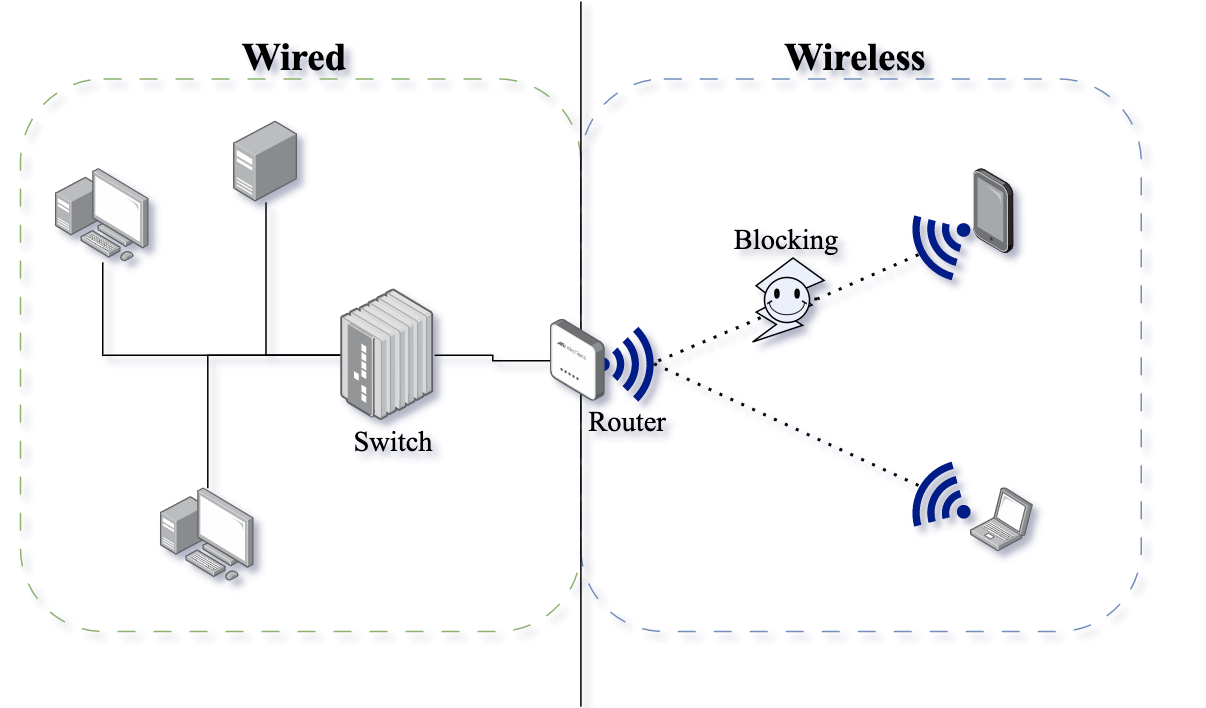
\includegraphics[scale=0.65]{../diagrams/drawio/domains.png}
  	\caption{Example of network domains}
  	\label{fig:domains}
\end{figure}

Each domain has different requirements that a single TCP connection cannot satisfy. Fig. \ref{fig:domains} shows the two domains and their characteristic differences. Usually, wireless domains experience a lot of changes in connectivity and bandwidths, while the wired domain is usually considered stable. This creates problems for TCP which normally spans multiple domains. Especially congestion control has problems adapting to highly fluctuating bandwidth across long distances and multiple domains. 

\subsection{Congestion Control}
Congestion occurs in the internet when a network's resources, such as routers, are overloaded to the point that they diminish quality of the network~\cite{rfc6077}. Packet loss and delays are common issues associated to congestion in the network. To solve the problem of congestion, a distributed algorithm is used: Congestion Control. The main goal of congestion control is to maintain a stable network, while still utilizing the available bandwidth shared among all flows. This is achieved by for example: additively increasing the sending rate, and multiplicatively reducing the sending rate when detecting congestion~\cite{welzl_congestion}. Congestion can be detected by monitoring packet loss, changes in delay, but also by explicit notifications.\\

Over time different variations of congestion controllers have emerged. Although their goal is the same: reduce congestion in the network, their approaches vary. Here are three examples:

\begin{itemize}
  \item \textbf{TCP Reno}: Reno embodies the traditional approach to congestion control: slowly increasing the sending rate while the network is stable and drastically reducing it on packet loss. TCP Reno was designed for unstable and dynamic networks, where the rapid response rate is crucial to prevent network overloading. However, the slow start rate and aggressive reduction of the sending rate make it sub optimal for more stable networks\footnote{This is not true, its bad with high BDP}, where packet loss is less frequent and predictable. Consequently, TCP Reno's reliance on packet loss may lead to unnecessary rate reductions and decreased network throughput.
  \item \textbf{Vegas}: Vegas is similar to TCP Reno in most aspects, the main difference is the use of delay to detect congestion instead of packet loss. This makes New Vegas able to react faster to congestion, however it also introduces some problems. If Vegas competes with TCP Reno flows, it will start reducing its sender rate before TCP Reno does, this leads to Vegas losing out on possible bandwidth. 
  \item \textbf{Cubic}: Cubic improves on the idea of TCP Reno by using a cubic function to adjust its sending rate in order to achieve higher throughput in a fast manner. Cubic is very efficient in highspeed networks and known for handling large data transfer over long distances. However, Cubic is not as reliable and robust as more traditional congestion controllers like TCP Reno.\footnote{Find source, reason for this sentence is that the window changes  more radically?}
\end{itemize}

In summary, the main differences between TCP Reno, Vegas and Cubic are their approach to congestion control, their performance in different types of networks, and their trade-off between efficiency and reliability.

\subsection{3 Way handshake (0 RTT)}
For TCP to establish a connection it uses a three-way handshake. Initially, it transmits a synchronization (SYN) packet to the desired endpoint. The endpoint responds with an acknowledgement and a synchronization packet of its own (SYN/ACK). Finally, the client responds with a acknowledgment (ACK). At this point both endpoints have confirmed that they are ready for further communication. For any connection to be established this handshake has to be done. For short flows that terminate in just a few round trips the initial TCP handshake can be a bottleneck, which is made worse if the connection is using a proxy\footnote{Proxies have not been introduced, can I assume people know what a proxy is?} and has to exchange additional information. 

\begin{figure} % htbp stand for "here", "top", "bottom", "page"
	\centering
	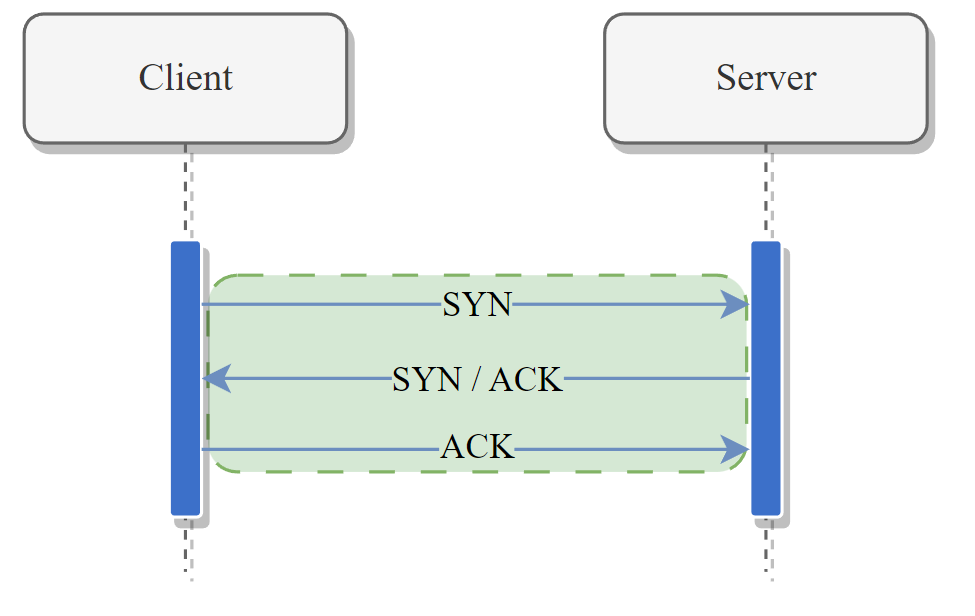
\includegraphics[scale=0.75]{../diagrams/drawio/tcphandshake.png}
  	\caption{The TCP handshake procedure}
  	\label{fig:tcphandshake}
\end{figure}

\subsection{TCP Options and Fast Open}
A TCP connection can be configured with optional header extensions called TCP Options~\cite{tcp_options}. These options change the default behaviour of TCP or add new features. One such feature is TCP Fast Open, which allows data to be added to the initial synchronization packet. A typical use case could be adding a HTTP GET request, thereby saving an entire round trip. In general, flows that terminate in a few round trips greatly benefit from this feature because the bottleneck is within the initial TCP handshake. Therefore, by removing the extra round trip required to send the first data packet, a significant amount of time can be saved.\\

TCP Fast Open also has other benefits, such as establishing connections to proxies~\cite{rfc8803}. When one is establishing a connection through a proxy, one gets the added delay of a second round trip for sending the desired endpoint. This can be avoided by using TCP Fast Open to send the desired endpoint in the first synchronization packet to the proxy. "SYN forwarding" enables the users to establish a proxy connection without any added delays, however it does depend on the user's application to use TCP Fast Open.

\section{The future of wireless communication.}
Wireless communication has seen a lot of improvements such as highly increased bandwidth achieved through advanced technologies like 5G. Millimetre frequency bands have opened up new possibilities for wireless communication. These higher frequency bands offer greater capacity and can accommodate more devices, however high frequencies come with a set of new challenges such as highly fluctuating bandwidths. This fluctuation can be influenced by various factors such as signal interference, obstacles in the signal path, and environmental conditions.

\subsection{5G Millimetre Wave}
The emergence of 5G Millimeter wave communications has opened the doors for low latency networks with multiple gigabits bandwidth. This is achieved by using higher millimetre wave (mmWave) frequencies in the range of 30GHz to 300GHz, which has a lot of benefits~\cite{Agrawal_Sharma_2016}. A wider spectrum of frequencies to choose from and higher data transfer rates are just some of the many benefits mmWave provides. But alongside the benefits, mmWave has also introduced a lot of new challenges.\\

A big problem with millimetre wave communication is signal path blocking, also called "Line of sight blocking"~\cite{mmwave_blocking}. It's caused by the use of Beam-forming to increase the bandwidth and range of milimeter wave signals. Beam-forming focuses the signal in a certain direction, making any blocking of the signal path devastating for the bandwidth. Even the human body can create enough blockage to drastically reduce the bandwidth. This causes huge fluctuations in the bandwidth whenever the signal is blocked.\\
\begin{figure} % htbp stand for "here", "top", "bottom", "page"
	\centering
	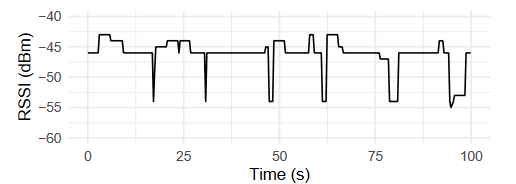
\includegraphics[scale=1.25]{../diagrams/graphs/tcp_mmwave_blockage.png}
  	\caption{5G bandwidth fluctuations from humans}
  	\label{fig:blockage}
\end{figure}

Fluctuating bandwidths lead to unstable TCP connections with a worst case of losing packets. Current TCP congestion controllers such as CUBIC, Reno or Vegas struggle when reacting to sudden changes.\cite{bandwidth_changes} They are simply not able to utilize the high bandwidth when it is available. Increasing the aggressiveness of a congestion controller is not an option either, as it would disrupt the internet. A possible solution could be to buffer packets at the 5G base stations, having the data ready for when the bandwidth is high. This however creates a new problem: "bufferbloat".


\subsection{Buffering}
\subsubsection{Bufferbloat}
The bufferbloat problem occurs when the systems between the endpoints buffer so many packets that the latency drastically increases and the reliability of the network as a whole goes down. The increased latency is detrimental for interactive (latency sensitive) applications. Generally it's preferred to drop packets and keep buffers small to avoid buffering time sensitive packets such as synchronization packets. Although this works in most cases, it's far from a optimal solution.\\

The increased bandwidth and low latency promises of new technology such as 5G has put a lot of pressure on the efficient forwarding of packets. Small buffers are therefore the standard, but at the same time, fluctuating bandwidth has shown the potential need to buffer packets for non-interactive traffic.
Most focus has been on accommodating latency sensitive applications like virtual reality or remote surgery to name a few.\\\\
This thesis will explore non-interactive applications where latency is not that critical and more buffering is acceptable and most likely desirable. By splitting traffic into interactive and non-interactive we can improve the performance of both. By having very small buffers for interactive applications we avoid bufferbloat problems, while utilizing the benefits of big buffers for non-interactive applications.\\

\subsubsection{Active Queue Management}
Active Queue Management (AQM) is about managing the length of queues in a network. By dynamically adjusting the queue length, AQM algorithms\cite{aqm_survey} prevent the buffer from becoming too full or too empty\cite{aqm}. This proactive management ensures smoother traffic flow and reduces the chances of packet loss or delay. AQM serves as a concept for more advanced techniques like packet scheduling, which further refines the process of handling network traffic.

\subsubsection{Packet Scheduling}
Another method of reducing the effects off bufferbloat is packet scheduling. A system should not send more packets than the weakest link can handle; this idea is built into TCP in the form of congestion control. However, when buffers grow to the point of causing bufferbloat, TCP's congestion control algorithms are unable to confidently determine a sending rate. Packet scheduling can solve this problem as it also controls the size of the buffers. It makes sure queues can grow when needed, but keeps the overall state of the buffers low. Packet scheduling has a lot more to offer than simple queue management, this will be explored later.\\

Proposed algorithms:
\begin{itemize}
  \item \textbf{FQ\_CoDel}: The Flow Queue Controlled Delay algorithm, FQ\_CoDel for short, was developed to deal with the bufferbloat problem. Its main goal is to reduce the impact of head-of-line blocking and give a fair share of bandwidth by mixing packets from multiple flows~\cite{fq_codel_rfc}. Internally FQ\_CoDel uses a FIFO queue, classifying packets into different flows to provide a fair share of bandwidth.
  \item \textbf{HTB}: Hierarchical Token Bucket is a queuing discipline based on assigning different classes a certain amount of bandwidth and sending rate. Because of its extensive bandwidth and delay management it's a good option for testing, especially in a virtual environment.
\end{itemize}

\subsection{Non-Interactive Applications}
Non-Interactive applications such as web traffic, file transfers and video streaming can benefit from larger buffering, especially with fluctuating bandwidths. This is because, if we are able to buffer the packets closer to their final destination, we have them ready to be sent when the bandwidth changes. As this thesis will show, by buffering them we can decrease delay times and achieve faster total completion times for non-interactive traffic.(need citation or prove it myself?). At the same time, with the solution presented in this thesis, interactive applications will not suffer under large queue delays that occur under normal buffering.

\section{Proxy}
Proxy servers play a big role in the modern internet, delivering benefits such as anonymity and increased performance~\cite{nextgen_proxy_servers}. A common use case for a proxy is caching by keeping a copy of popular resources such as a websites. This reduces the latency of accessing the resource as long as the proxy is closer to the user than the original copy. Locality plays an important role in the total latency as any transmission will always be limited by the speed of light.\\

A proxy can also be used for privacy similar to a Virtual Private Network (VPN). By redirecting network traffic through a proxy, the origin of the traffic appears to be the proxy server rather than the actual end-user. Hypertext Transfer Protocol (HTTP), a popular internet protocol used for accessing websites, has this functionality built in using HTTP tunnels and a special CONNECT method in its header:\\

\begin{verbatim}
CONNECT mn.uio.no/:22 HTTP/1.1
Proxy-Authorization: Basic encoded-credentials
\end{verbatim}

\subsection{PEP}\footnote{Include that they need to be on path to be "fast"}
A performance enhancing proxy (PEP) is a proxy designed to increase the performance of applications using it, typically by influencing the behavior of TCP. The idea behind the PEP is putting more logic, such as connection management, buffering, caching inside the network. As the name suggests, a PEP is designed to enhance the performance, but can also introduce new features to a network. An example of a new feature is the multipath support the TCP Transport converter gives~\cite{rfc8803}.

\subsection{PEP for wireless communication}
Performance enhancing proxies are already deployed and in use for a lot of wireless communication, especially satellites and radio access networks~\cite{tcp_mmwave_proxy}. They have an inherent performance increase just by splitting the connection between the wireless and wired domains. These PEPs are therefore often installed at the base stations. However they are unable to distinguish between interactive or non-interactive traffic, meaning their buffers need to be small to avoid bufferbloat and hence why still suffer from fluctuating bandwidth problems.\footnote{Confusing sentence?} Alternatively, a PEP with a large buffer can compensate for fluctuating bandwidth, but will introduce delay for interactive traffic.

\begin{figure}[h] % htbp stand for "here", "top", "bottom", "page"
	\centering
	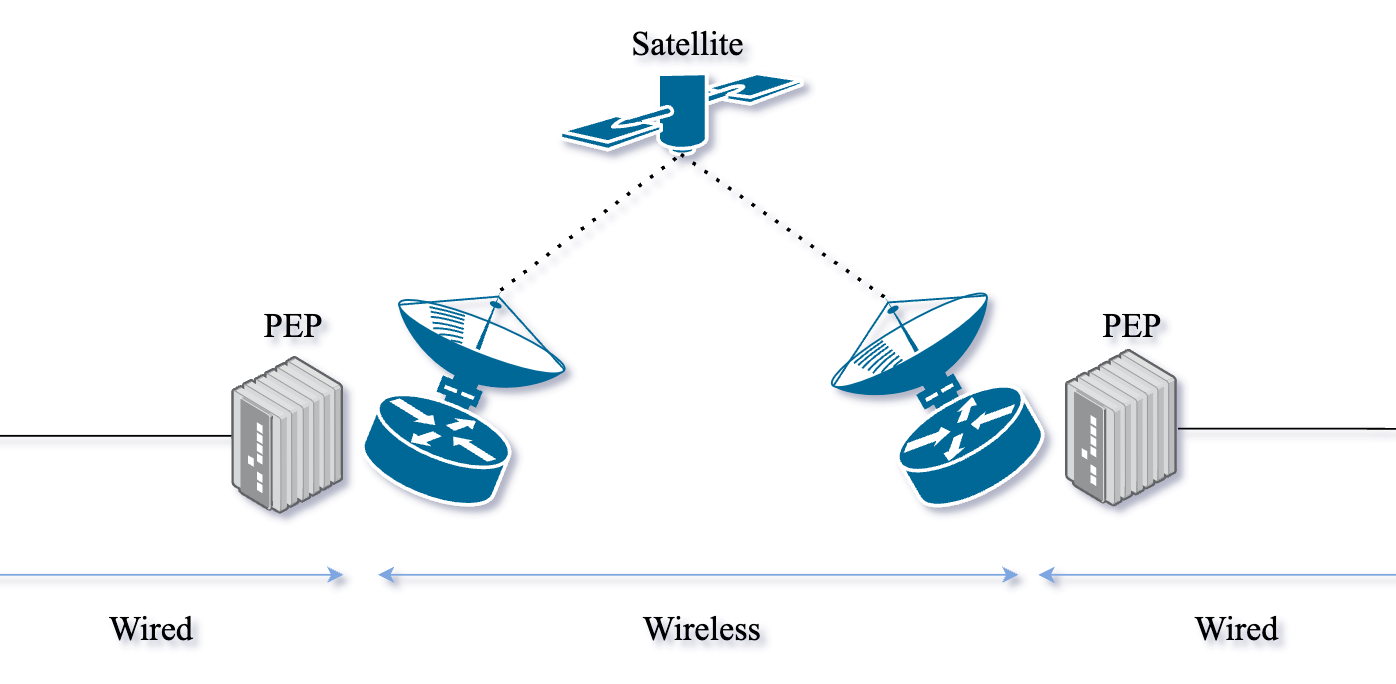
\includegraphics[scale=0.50]{../diagrams/drawio/pep_satellite.png}
  	\caption{PEP installed to support Wireless traffic over satellite.}
  	\label{fig:blockage}
\end{figure}

\subsection{Transparent vs Non-Transparent}
A big discussion regarding PEPs has been if they should be transparent or non-transparent. Transparent PEPs are not visible to the applications that use it. They silently split the connections and spoof the IP-address of both the client and server~\cite{pep_dna}. This is prone to cause unintended side effects, such as certain TCP options not being forwarded, and security concerns. Non-Transparent PEPs on the other hand are explicitly chosen by either the client or the server, and the sender is aware of the proxy splitting the original connection. This approach can be seen as more appropriate for the internets architecture and could potentially remove some of the stigma associated with PEPs. This however requires modifications at the sender side to utilize the PEP.

\section{Linux}

Linux is the most famous open source kernel freely available for anyone to use and modify. Because of the open source nature of Linux, there have been many operating system implementations based on the Linux kernel. Ubuntu, Fedora or Manjaro are just some of the most famous Linux based operating systems out there. For developers, Linux is the perfect platform to experiment and test their new innovations. One is able to modify and recompile the kernel itself on the fly, and then test the solution on a live operating system. Linux supports most standards and is used by most major corporations such as Facebook, Amazon, Netflix and Google.

\subsection{Kernel Modules}
A concept that makes Linux truly extensible are Loadable Kernel Modules (LKM). Kernel modules are programs that can be loaded at runtime into the kernel and run with kernel privileges. Running with kernel privileges has a lot of benefits such as having access to internal structures and kernel symbols. Most drivers in the Linux kernel are written as kernel modules as they need access to the system internals.\\

Congestion controllers and packet schedulers are also usually implemented as kernel modules. That is because Linux exposes a struct with function pointers that can be overwritten by a module, making the kernel call the new functions instead. Because kernel modules run as part of the kernel they do not need to use a system call to do basic I/O as using sockets. Removing the overhead of system calls makes the kernel modules run much faster than default user space programs.\\

However, using Linux kernel modules has the drawback that the program is bound to Linux. The modules will only work in the context of the Linux kernel as they depend on the internal functions, and that they are part of the kernel. Most other operating systems like MacOS will not allow user defined modules to run with kernel privileges. Additionally, any bugs or error in the kernel module with make the entire kernel fail ("panic"), which usually requires a complete system restart to fix.

\subsection{C Programming Language}
C has been the optimal language for high performance systems since its creation in 1972.~\cite{c_programming_language} It was originally created for UNIX when it needed a higher level language, and now is the main programming language behind most operating systems such as Linux, Mac and Windows. Being very close to its predecessor, assembly, and compiled to a binary, makes it one of the fastest languages we have to date. Heap memory management is explicitly done by the programmer with no support for garbage collection. The unsafe memory management is one of the main challenges when programming in C, which however can be a benefit because a runtime garbage collection usually results in performance loss.

\begin{autonumlstlisting}[label=lst:hello_world]{Default C program.}
#include <stdio.h>

int main(void)
{
	printf("Hello World!");
	return 0;
}

\end{autonumlstlisting}

\section{Related Work}
PEPDNA? 0RTT transport converter?\cite{bandwidth_changes}

% This chapter explores the design desgins that later will be implemented by chapter 4.
% Briefly outline the design goals of the PEP
% High-Level Architecture
\chapter{Design} %WHAT AND WHYs
In this chapter we discuss the design of a non-transparent connection splitting PEP at the boundary of an unstable network with fluctuating bandwidth, typically at 5G base-stations. By splitting the connection at this point we can buffer packets, usually closer to the user, and have them ready for high bandwidth phases. This is similar to how a content delivery network (CDN) stores caches and replicas closer to the users to reduce delay. The overarching goal is to improve the completion times of non-interactive traffic while avoiding to disturb the interactive flows that are passing through. A good design for the PEP is crucial as it needs to be robust, fast and reliable. \\

\begin{figure} % htbp stand for "here", "top", "bottom", "page"
	\centering
	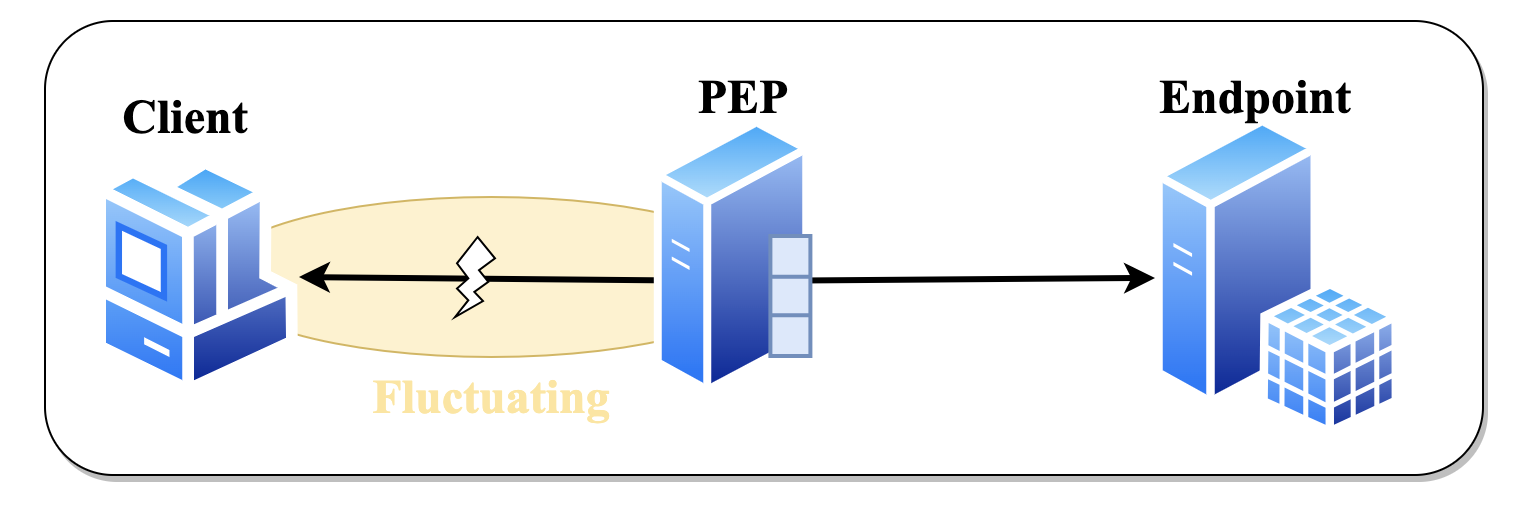
\includegraphics[scale=0.45]{../diagrams/drawio/simple_pep_design.png}
  	\caption{PEP within a network (Simplified)}
  	\label{fig:simple_pep_design}
\end{figure}

Figure \ref{fig:simple_pep_design} is a simplification of the PEP within a network, highlighting its interaction with other components, such as the client and endpoint. Importantly there is a fluctuating bandwidth between the client and the PEP.

\section{Justification for designing a PEP}
The ossification of networks, particularly TCP, has been a long-standing issue~\cite{tcp_extendable}. Over the years, the internet has evolved, but the core protocols, like TCP, have remained relatively unchanged. This leads to challenges when attempting to introduce extensions or modifications. Altering such a fundamental protocol could disrupt countless systems and applications. Which leaves us to explore new ideas using middle-boxes. A PEP is such a middle-box, as it can enhance the performance without introducing changes to TCP itself.\\

Using a PEP in combination with 5G has additional benefits. TCP with 5G needs to cover both the stable network and the fluctuating wireless domain split by the base station illustrated by figure \ref{fig:5g_topology}. However, with a PEP we are able to split the domains and perform optimizations such as congestion control and buffering, tailored to each specific domain. Achieving the same optimization by modifying TCP would need a change to the tight integration of end to end congestion control.\\

\begin{figure}[h!] % htbp stand for "here", "top", "bottom", "page"
	\centering
	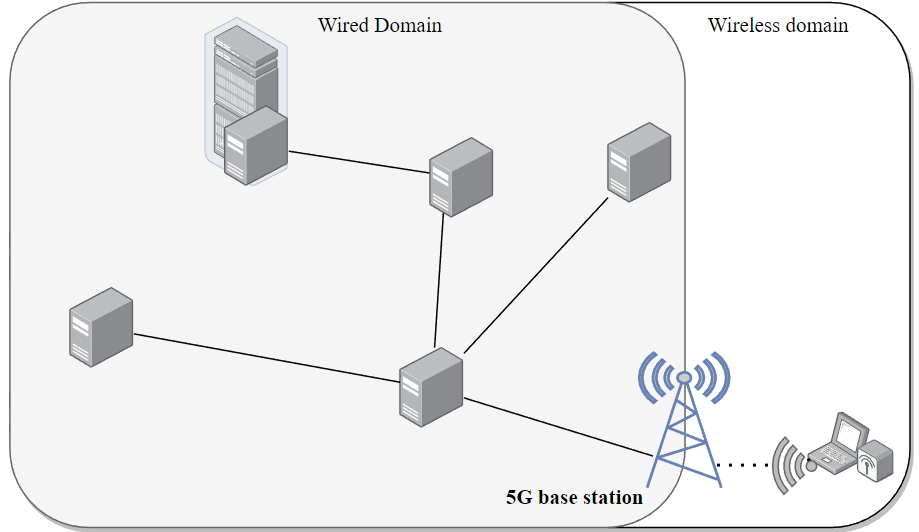
\includegraphics[scale=0.6]{../diagrams/drawio/deployment_without_pep.png}
  	\caption{Example 5G network topology}
  	\label{fig:5g_topology}
\end{figure}


\section{Performance}
In this section, we discuss the core design decisions to optimize the PEPs performance.
The speed at which a PEP can both process and forward packets is crucial. Especially when wanting to utilize the rapidly fluctuating bandwidth of 5G, we need to react as fast as possible. The design choices presented in this section focus on the performance of the PEP. Because of these high performance requirements, the PEP is written in C as a Linux kernel module. 

\subsection{Programming Language}
The programming language chosen for a PEP has a direct impact on its efficiency. Interpreted languages like Python might not offer the speed necessary for high-performance tasks. Even Java, while running within the JVM with JIT and garbage collection, can potentially introduce delays. The languages best suited for high performance are C, C++ and Rust. Both C and C++ are very similar and well suited for high performance systems. The reason for choosing C is its bare metal approach and integration into the Linux kernel with kernel modules.

\subsection{Kernel Module Vs. Userspace Application}
When sending data over the network, all calls to receive and send data has to go through the kernels internal network stack. These calls are usually in the form of system calls when running as a user-space application. Making system calls (syscalls\footnote{Section about system calls?}) can introduce a lot performance overhead in the form of a context switch to kernel-space and copying data back and forth from user-space to kernel-space. A kernel module will be able to directly access the kernel functions, eliminating the overhead of system calls and the restricted access of userspace applications to the network stack.\\

Opting for a user-space application has the advantage of being cross-platform, meaning it can run on multiple operating systems without major modifications. In contrast, kernel modules are tightly bound to the Linux environment, which might limit its usability to Linux hosts. This however is not a big problem as most servers are Linux hosts. [CITE]

\subsection{Connection splitting using Sockets}% WHAT AND WHY
% Talks about splitting domains 
The PEP uses sockets to establish and split the connection between the client and the endpoint. Sockets provide a standardized way for programs to send and receive data over a network. They act as communication points, allowing for data exchange between them. For the PEPs purpose, sockets are ideal because they are configurable and come with dedicated buffers. This makes it easier to split and manage connections efficiently. Additionally, sockets are widely supported, ensuring compatibility and ease of integration~\cite{ibm_doc}.\\

A connection splitting proxy has the benefit of additionally splitting the connection into different domains. As discussed in Chapter 2, the internet consist of different domains with their own characteristics. Being able to split the connection into their different domains, enables the PEP to adapt and select an appropriate congestion controllers based on the technology and topology of each domain.\\

Each socket connection can be configured to use a certain congestion controller, unrelated to the system wide default. Which would be impossible with a single end to end connection. In addition to configuring the congestion controller, a socket can also add TCP options, such as TCP Fast Open, to a connection.

\subsection{Bandwidth utilization}
Another great benefit of connection splitting is potentially better bandwidth utilization. When using congestion control: the total bandwidth is usually determined by the lowest bandwidth on the path\cite{top_down}. This is done to prevent overwhelming the link with the lowest bandwidth, as doing so would lead to congestion along the network path. Figure \ref{fig:pep_bandwidth_bad} shows a theoretical path between host A and host D, there are two links with high bandwidth, 60 Mbps and 75 Mbps. But because of the last link between C and D, the total bandwidth between A and D is 15 Mbps. This leads to a 25\% bandwidth utilization of link AB and 20\% utilization of link BC.\\

\begin{figure}[h!] % htbp stand for "here", "top", "bottom", "page"
	\centering
	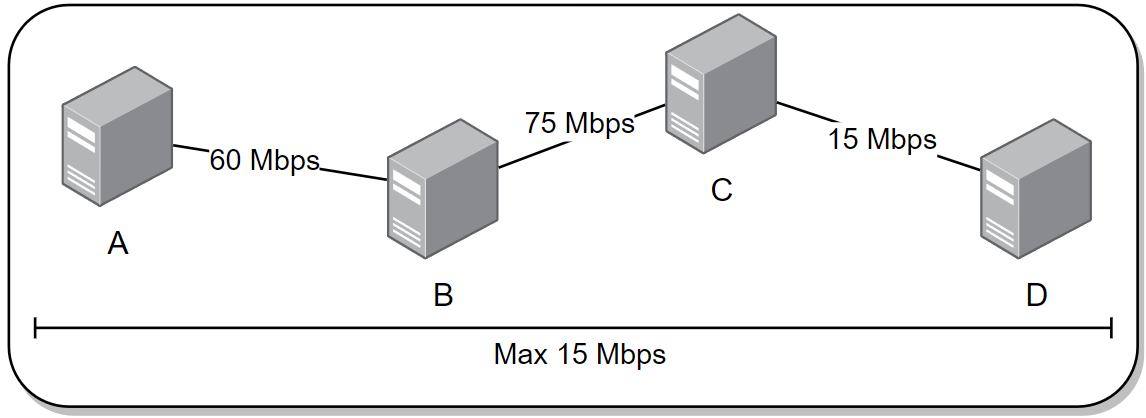
\includegraphics[scale=0.45]{../diagrams/drawio/bandwidth_bad.png}
  	\caption{Example of poor bandwidth utilization.}
  	\label{fig:pep_bandwidth_bad}
\end{figure}

Figure \ref{fig:pep_bandwidth_good} shows the same path as Figure \ref{fig:pep_bandwidth_bad}, however there is a connection splitting PEP at C. In that scenario we get two total bandwidths, one for each connection. The first connection between A and C has a total bandwidth of 60 Mbps, while the connection between C and D remains at 15 Mbps. Looking at the bandwidth utilization we now have 100\% utilization on link AB, 80\% utilization at BC. Which is a major improvement from the original 25\% and 20\% utilization.

\begin{figure}[h!] % htbp stand for "here", "top", "bottom", "page"
	\centering
	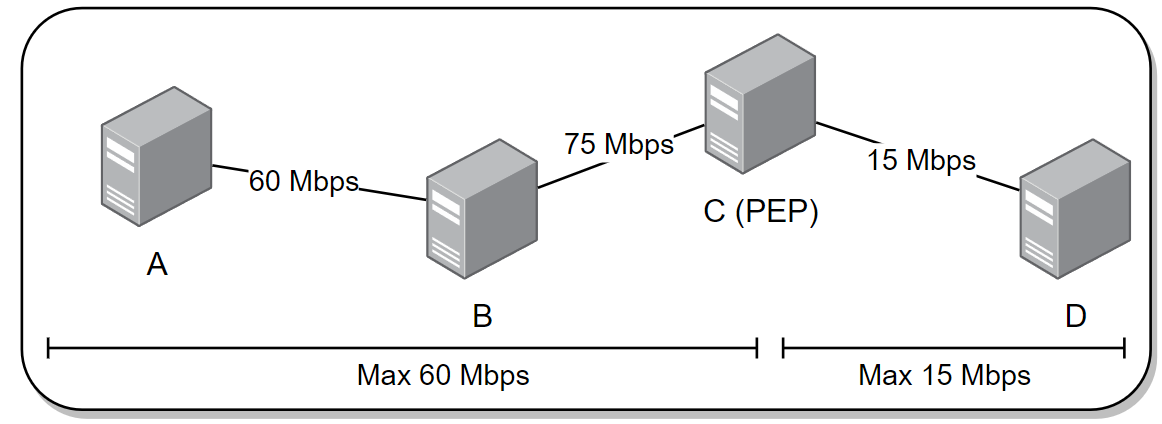
\includegraphics[scale=0.45]{../diagrams/drawio/bandwidth_good.png}
  	\caption{Example of good bandwidth utilization.}
  	\label{fig:pep_bandwidth_good}
\end{figure}


\begin{table}[h!]
\centering
\begin{tabularx}{\linewidth}{lCCCCC}
\toprule
Link & Without PEP & With PEP \\
\midrule
AB & 25\% & 100\%\\
BC & 20\% & 80\% \\
CD & 100\% & 100\% \\
\bottomrule
\end{tabularx}
\caption{Table showing bandwidth utilization with and without a PEP.}
\label{tab:pep_bandwidth_table}
\end{table}


\paragraph{Delay}
Table \ref{tab:pep_bandwidth_table} gives an overview of the bandwidth improvements. However, even with the improvement of bandwidth utilization, we did not improve the end to end throughput from A to D as it is still limited by link CD. An important component is missing: Delay. Looking at the topology of Figure \ref{fig:pep_bandwidth_good}, we can assume an inherent lower delay between C and D, because of locality, than between A and D. If we now introduce a fluctuating bandwidth on the link CD the lower delay between C and D means the congestion controller can react faster.\\

\begin{figure}[h!] % htbp stand for "here", "top", "bottom", "page"
	\centering
	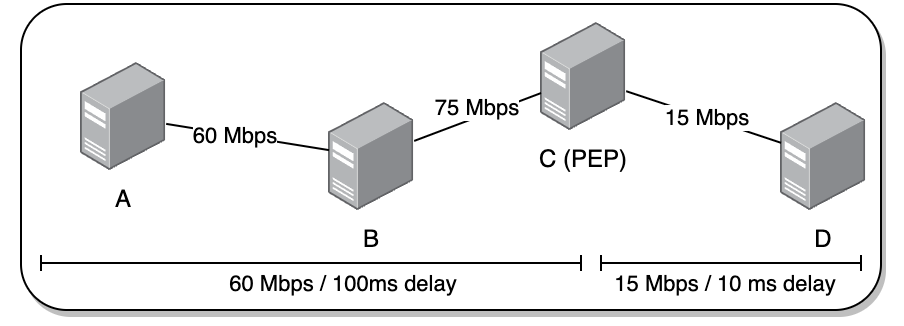
\includegraphics[scale=0.6]{../diagrams/drawio/bandwidth_delay.png}
  	\caption{Split connection with bandwidth and delay.}
  	\label{fig:pep_bandwidth_delay}
\end{figure}

Figure \ref{fig:pep_bandwidth_delay} introduces delay to the topology. Without the PEP we would have a end to end connection with 15 Mbps and 110 ms delay (220 ms RTT). Assuming the bandwidth on the link between C and D is highly fluctuating, the TCP congestion controller needs 220 ms for each round trip to react. However, if we split the connection at C, the time would be reduced to 20 ms. This means the congestion controller, between C and D, can react 1000\% faster with a split connection. Thereby better utilizing the fluctuating bandwidth.
 
\subsection{PEP Selection}
The connection process to the PEP, and later on the endpoint, is established by informing the PEP of the desired endpoint of the client. This can be achieved by a variety of ways where the goal is to attach additional information to the default connection process of TCP. Preferably, we do not want the overhead of needing an entire additional round trip just to pass this information. Figure \ref{fig:tcphandshake_primitiv} visualizes the RTT overhead of sending this information (in red) to the PEP before application data can be sent.\\

We do not want to change the normal socket based scheme of creating a connection either, as old applications would need to rewrite a lot of their code to adapt a new scheme. By providing a library for the client we can easy the challenges of integrating the PEP into existing environments. The library will provide a single function which mimics the default connection scheme. Implementation details are discussed in Chapter 4.

\subsection{Connection Establishment}  
The PEP will attach data to the initial TCP handshake, this way we can inform the PEP of the endpoint without needing to send it with an additional round trip time. Because of the ossified nature of TCP~\cite{tcp_extendable}, changing the protocol itself is not an option. The realistic approach is reusing existing TCP functionality to append the desired data. Only a small amount of data, less than the usual Maximal Transmission Unit (MTU), is needed to inform the PEP of the endpoint. \\

\begin{figure} % htbp stand for "here", "top", "bottom", "page"
	\centering
	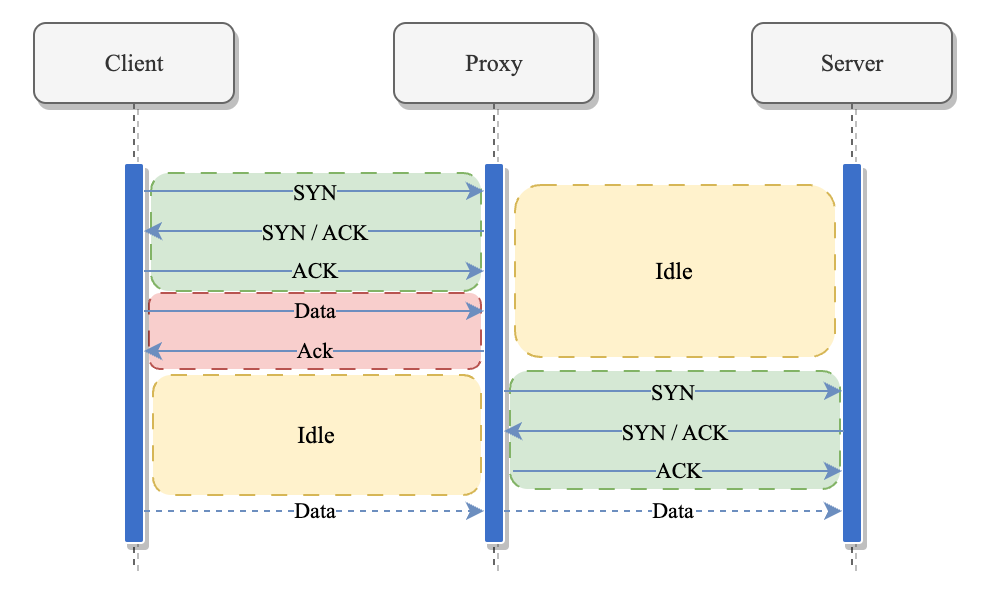
\includegraphics[scale=0.75]{../diagrams/drawio/tcphandshake_primitiv.png}
  	\caption{The TCP handshake procedure across PEP}
  	\label{fig:tcphandshake_primitiv}
\end{figure}

\paragraph{TCP Options}
Since TCP Options can be attached to a TCP connection, a possibility would be to add a new TCP Option which would specify the endpoint. This TCP Option would need to be added by a kernel module, as it is not possible to to add custom TCP Options from user-space. This leads to another problem, mainly how to specify from user-space that we wish to use the PEP.\\

A possible option would be a socket option, using setsockopt. This however requires changes to the kernel, which raises the bar for adaptability. Another choice would be always attaching the TCP Options on connection addressed to a certain port such as 80/443. This however takes away the choice from the application, and makes it system wide instead.\\

Finally, another significant problem is that unknown TCP Options are often seen as a threat. Firewalls may drop the packets, or the options might be stripped by intermediate nodes~\cite{middlebox_interactions}. This creates a challenge for the implementation and usability of the PEP. If the packets may be dropped because of our custom TCP options, then the PEP will only work in certain networks and scenarios. Although we only design a proof of concept, this is a trade off that is unlikely to pay off in the end~\cite{tcp_extendable}.

\paragraph{TCP Fast Open}
Another possibility is using the existing TCP Fast Open option which can attach data to the initial TCP handshake. As discussed in the Chapter 2, using TCP Fast Open can reduce the amount of RTTs needed to establish a connection with both the PEP and endpoint. This requires the socket to be configured and enabled system-wide on the server machine. TCP Fast Open is also fault tolerant. Should either the PEP or the client not support TCP Fast Open, the meta-data will still be sent with the cost of an additional RTT. 

\paragraph{Optimal Choice}
The most sustainable choice is TCP Fast Open, as adding new TCP Options is simply too unstable. Also, the goal of our PEP is not to change or extend TCP itself. Using TCP Fast Open also has the advantage of being able to add meta data in the size of an MTU, which adds to the adaptability of the PEP to be extended in the future.\footnote{Rephrase last sentence.}\\

\begin{figure} % htbp stand for "here", "top", "bottom", "page"
	\centering
	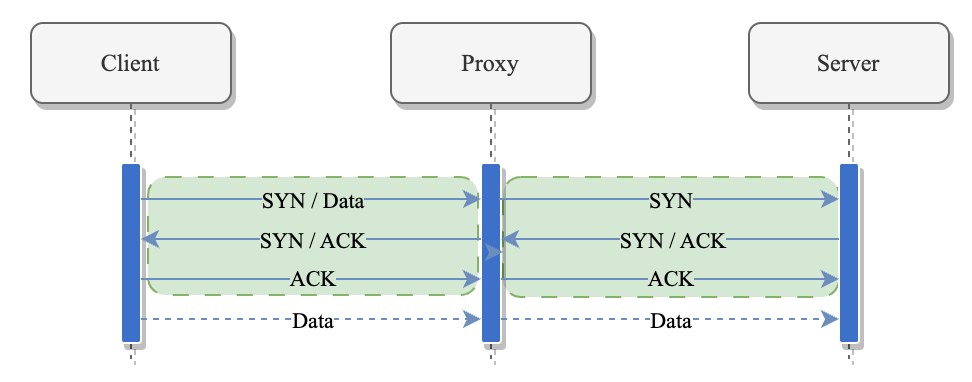
\includegraphics[scale=0.75]{../diagrams/drawio/tcphandshake_optimal.png}
  	\caption{Optimal handshake across PEP (0 RTT)}
  	\label{fig:tcphandshake_optimal}
\end{figure}

Figure \ref{fig:tcphandshake_optimal} shows the concept of the added data to the TCP handshake, reducing the idle time visualized in Figure \ref{fig:tcphandshake_primitiv}. 

%\subsection{Optimal Choices for PEP Performance}
%Because of the efficiency and possibilities of kernel modules, C offers the optimal performance for the %PEP. This combination leverages C's high-speed capabilities and the direct kernel integration, %minimizing overheads and maximizing efficiency. This choice binds us to the Linux kernel, but this is a %small price to pay for salvation.\footnote{Find a actually good way to say this. :) Also! Future work %could be comparing to a user-space application? }

% This is a overaching design choice, not a implementation specific. 
% So the text will be more about WHY
\section{Deployment (Transparency)}
The deployment of the PEP is an important design aspect. In this context, deployment refers to the physical location of the PEP. The main factor which affects deployment is the transparency, Chapter 2 quickly discussed the differences between the two approaches. This section will discuss the differences in the context of our PEP, especially in combination with wireless networks.

\subsection{Transparent PEP}
Transparent PEPs provide a deployment advantage since they can be integrated without altering the client or server. This means even older applications can utilize the PEP. Moreover, the PEP will inherently be on the same path as the original connection, which is a prerequisite for a PEP. But, if unknown middle boxes interfere with a connection, issues like lost TCP Options might occur. Additionally, if applications are not aware of the PEP, they can not adjust their behavior, restricting their future adaptability.\\

Most transparent connection splitting PEPs spoof the IP address of the original endpoint. From the perspective of the client, it is talking to the actual endpoint. This may lead to issues, as several assumptions held by the client may no longer be valid. One assumption is that when I receive an ACK, the associated data segment was successfully received by the endpoint. But since the PEP is pretending to be the endpoint the ACKs only mean that the PEP received the data, not the endpoint. If the PEP would crash any data which the PEP has buffered would be lost. This would mean that the client assumes that the endpoint received the data, even though it did not.

\subsection{Non Transparent PEP}
In contrast, with a non-transparent PEP the deployment is more difficult. When a client needs to explicitly choose the PEP, it also needs to know that the PEP is on the path to the desired endpoint. Normally this would be extremely difficult to achieve. But, because the PEP is designed to be deployed at the base stations of wireless networks, such as 5G, we can assure that all traffic will pass through it. Thereby being on inherently on path and eliminating the deployment problem of non-transparent PEPs.\\

Although non-transparent PEP still may crash and buffered data may be lost. There is no assumptions by the client that the data was delivered to the endpoint. Clients are aware of the potential failures that may occur when using a PEP, similiar to using a VPN. Non-transparent PEPs are more sustainable as they avoid the need to spoof IP addresses and include the clients which lets them adapt and avoid invalid assumptions.\\


\begin{figure} % htbp stand for "here", "top", "bottom", "page"
	\centering
	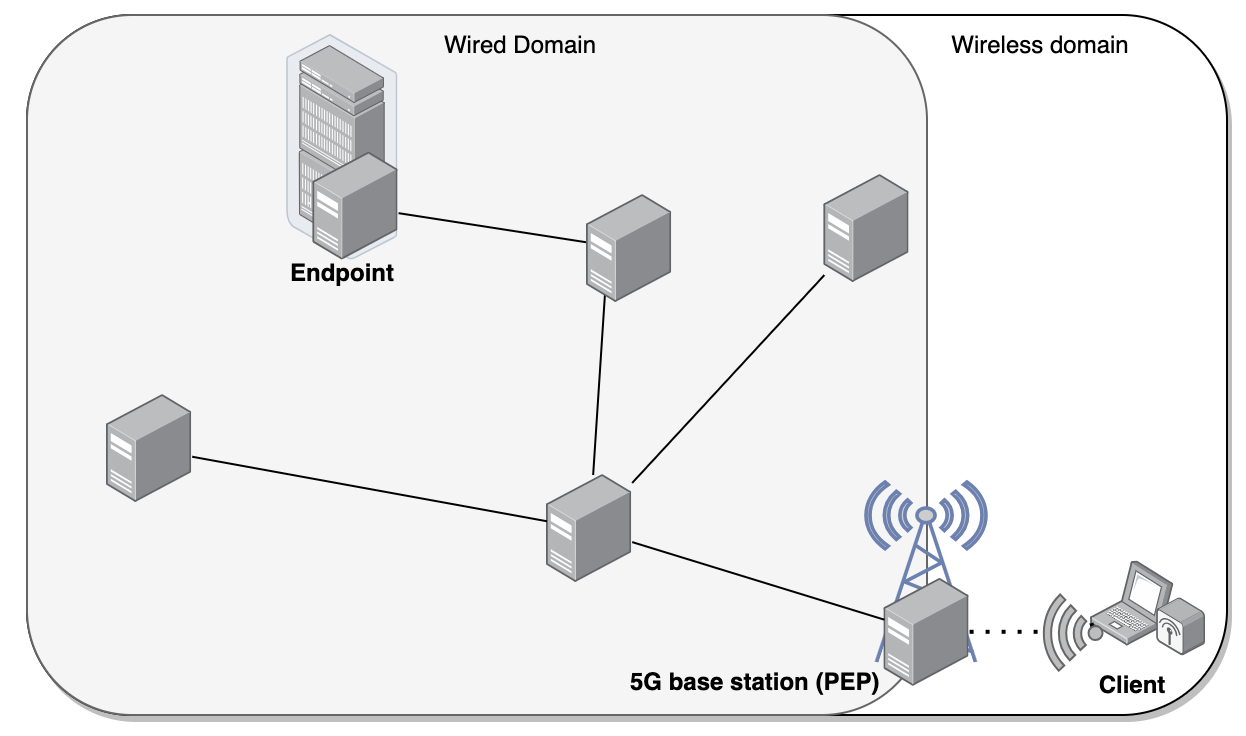
\includegraphics[scale=0.55]{../diagrams/drawio/deployment.png}
  	\caption{Deployment of a PEP at a base station}
  	\label{fig:pep_deployment}
\end{figure}


Since applications are fully aware of the PEP when it is non-transparent, we can adjust the PEPs functionality based on the application using it. Applications can also adapt their behaviour, optimizing their operations based on the presence of the PEP, leading to additional performance improvements. Although side effect may still occur, applications are aware of them and can actively mitigate them.\\

This thesis will utilize a non-transparent PEP located at a base station. Mostly for the benefits of future adaptability and the client being aware of the PEP. Being located at the base station assures that the PEP will be on path, which normally is a major challenge for non-transparent PEPs.

\section{Buffering}
Buffering is a core feature of the PEP. As mentioned before, the goal is to buffer non-interactive traffic packets at the PEP. Normally the context of buffers in the network, revolve around NIC buffers or routing buffers. Those buffers affect all traffic passing through and will cause Bufferbloat if the buffers are too large. That's why, normally, the goal is to keep these buffers low to avoid disturbing interactive traffic. However, since the PEP is using sockets and splitting the connection, we can utilize a different buffer: the socket buffers.

\subsection{Socket buffers}
A socket buffer is a buffer specific for a particular socket. There are usually two buffers, one for read on the socket and one for write. This offers a great opportunity for buffering only a certain type of traffic, as a socket buffer does not affect traffic which flows through the host machine. A connection splitting proxy inherently has two sockets, one for the client and one for the endpoint. Which means we get a total of 4 buffers per 'flow', each individual read and write buffer can be configured for the best performance.

\section{AQM \& Scheduling}
The ability to configure and utilize different scheduling algorithms is important for the success of the  PEP. When buffering a lot of packets at the PEP we might clog up the sending queues of the host machine. This would result in high delays for the interactive traffic who has to share these queues with our buffered non-interactive data. To avoid this we utilize FQ\_CoDEL, as it assures a fair bandwidth for each flow.\\

This is another choice which will bind us to Linux, as achieving the same control and configuration on other operating system, such as Windows or MacOS, will be extremely difficult or even impossible. The impact of different scheduling algorithms will be shown and discussed in the Evaluation chapter.

\section{Security}
The PEP needs to assure that traffic flowing through the PEP not gets compromised. This, however, will not be a big concern as the PEP will only forward application data, meaning higher level security protocols such as TLS will still be end to end. This assures that the PEP is not able to read encrypted data or be used for malicious intents. The PEP can have the additional benefit of hiding the identity of the user from the endpoint. As only the PEPs connection will be seen by the endpoint.

\section{Summary}
In this chapter we have designed a high performance connection splitting PEP tailored for fluctuating bandwidth. We made choice to keep it non-transparent to assure future adaptability and client configuration. Using sockets and their buffers we avoid bufferbloat and to not disrupt the interactive traffic. Finally, we use AQM and scheduling to avoid unnecessary delays on the outgoing links.\\

The table below compares our PEP to existing solutions. ...\\

\begin{table}[h!]
\centering
\begin{tabularx}{\linewidth}{lCCCC}
\toprule
Implementation & 0RTT & Connection Splitting & Special ACKs & Transparent \\
\midrule
\textbf{milliProxy} & AF & AFG & 004 & x \\
\textbf{PEPDNA} & AX & ALA & 248 & x \\
\textbf{SnoopTCP} & AL & ALB & 008 & x \\
\textbf{Our PEP} & DZ & DZA & 012 & x \\
\textbf{Transport Converter} & AS & ASM & 016 & x \\
... & AD & AND & 020 & x \\
... & AO & AGO & 024 & x \\
\bottomrule
\end{tabularx}
\caption{Table of design decisions based on different PEP implementations compared to ours.}
\end{table}

Most PEPs are transparent, this makes our PEP special...

% TRL TCP https://ieeexplore.ieee.org/abstract/document/4623710?casa_token=nB8IUC46VVQAAAAA:q9PoGtpzLJDUCfrjMzeAi9DG7VKQoSQVmogIdidf-ydVmt7e2ZtL5O1859WLVM6a_wXn_IZijFM

% HTTPPEP https://citeseerx.ist.psu.edu/document?repid=rep1&type=pdf&doi=137fd719d5aa77145b38397bbd5effb6de3ee1c9 


\chapter{Implementation}
This chapter will explore the implementation of the TCP PEP, following up on the design choices made in the previous chapter. The development of the PEP will give a deeper understanding of the underlying mechanisms and how they aim to better utilize the 5G bandwidth. All aspects from kernel modules, PEP architectures and additional libraries will be covered.

\section{Kernel Module}
As mentioned in the design chapter, the PEP will be written as a kernel module instead of a normal user-space program. Running and creating a kernel module requires more initial preparation than the a normal application. Firstly, the biggest difference is that our PEP will run as a module inside the Linux kernel instead of as a application in its own virtual environment. Injecting a module into the Linux kernel is very different from simply running a binary.\\

A Linux kernel module is loaded and unloaded with the help of two functions that need to be defined:\\

\begin{autonumlstlisting}[label=lst:module_example]{The basic kernel module setup code.}
/* Needed by all kernel modules */
#include <linux/module.h> 
#include <linux/kernel.h>
#include <linux/init.h>

/* entry function */
static int __init onload(void) {
    return 0;
}

/* exit function */
static void __exit onunload(void) {
    
}

module_init(onload);
module_exit(onunload);
\end{autonumlstlisting}

Listing \ref{lst:module_example} shows a basic kernel module, defining and exporting the functions onload() and onunload(). The name of the functions bear no meaning, the important parts are the macros \verb|__init|, \verb|module_init| and exit macros\cite{lkm}. When a kernel module is loaded the function declared with \verb|__init| is called.\\

Normally a application would terminate when it returns from its \verb|main| function. Kernel modules however remain "loaded" when returning from the initialization function. This brings us to a new paradigm when programming, instead of having a running program, we install hooks and callbacks which change the default behavior of the kernel. A callback architecture can be less resource intensive as we do not need threads polling for data.\\

A kernel module is loaded by first compiling it into a .ko file and then loading with the \verb|insmod| shell command:
\begin{verbatim}
$ insmod <module_name>.ko
$ rmmod <module_name>.ko
\end{verbatim}
The \verb|rmmod| is used to unload a kernel. 

\subsection{Kernel Hooks}
The Linux kernel exposes many function tables and callbacks which designate what functions to call at certain events. Most drivers and congestion controllers are implemented in this manner. A predefined struct is allocated and populated with custom functions, and installed with an existing kernel function.

\begin{autonumlstlisting}[label=lst:hook_example]{Example of a TCP congestion controller module}

static void my_init(struct sock* sk);
static u32 my_ssthresh(struct sock* sk);
...

static struct tcp_congestion_ops mycc __read_mostly = {
  .init           = my_init,
  .ssthresh       = my_ssthresh,
  .cong_avoid     = ...,
  .set_state      = ...,
  .undo_cwnd      = ...,
  .pkts_acked     = ...,
  .owner          = THIS_MODULE,
  .name           = "tuner",
};

/* entry function */
static int __init onload(void) {
    return tcp_register_congestion_control(&mycc);
}

/* exit function */
static void __exit onunload(void) {
    tcp_unregister_congestion_control(&mycc);
}

module_init(onload);
module_exit(onunload);
\end{autonumlstlisting}
In the Listing \ref{lst:hook_example} we demonstrate how a TCP congestion controller is implemented, in the context of a kernel module. This allows run-time modification of kernel behaviour, and is a programming paradigm\footnote{Is it a paradigm?} which will be useful to use when implementing the PEP.


\subsection{Linux Version and Distribution}
The kernel module was developed using Linux Kernel 5.15, older version of Linux might encounter problems as the kernel functions change a lot.

\subsection{Implications}

\begin{lstlisting}[caption={kernel\_recvmsg wrapper for receiving for TCP msgs}, label={lst:pep_tcp_receive} ,language=C]
int pep_tcp_receive(struct socket *sock, u8* buffer, u32 size)
{
	struct msghdr msg = {
		.msg_flags = MSG_DONTWAIT,
	};

	struct kvec vec;
	int rc = 0;

	vec.iov_base = buffer;
	vec.iov_len  = size;

	printk(KERN_INFO "[PEP] kernel_recvmsg: calling recvmsg \n");
pep_tcp_receive_read_again:
	rc = kernel_recvmsg(sock, &msg, &vec, 1, vec.iov_len, MSG_DONTWAIT);
	if (rc > 0)
	{
		tlv_print(buffer);
		printk(KERN_INFO "[PEP] kernel_recvmsg: recvmsg returned %d\n", rc);
		return rc;
	}

	if(rc == -EAGAIN || rc == -ERESTARTSYS)
	{
		goto pep_tcp_receive_read_again;
	}

	printk(KERN_INFO "[PEP] kernel_recvmsg: recvmsg returned %d\n", rc);
	return rc;
}
\end{lstlisting}

\section{TLV Library}
Regarding the endpoint addressing and selection by the client, a custom shared library is a good choice.
\footnote{Rewrite this.} The goal is to keep the client code as simple and close to its original form as possible, but still be able to communicate the desired endpoint, options and meta-data to the PEP. Additionally, we want to send this information by using TCP Fast Open which has a similar connection routine as default sockets do.\\

Normally a socket would first \verb|create|, \verb|connect| and then \verb|send| data using the \verb|send| system call. The creation of a socket is the same for both with and without TCP Fast Open. Which leaves us with connection as the main problem. The way we connect to a host using TCP Fast Open is by skipping \verb|connect| and instantly jump to \verb|sendto|. As we can see from the socket system calls, both \verb|connect| and \verb|sendto| take a \verb|struct sockaddr| as a parameter. A \verb|struct sockaddr| defines the endpoint to which you want to connect. \verb|sendto| has a flag option which allows the configuration of how messages are sent, and if we supply the \verb|MSG_FASTOPEN| flag, \verb|sendto| will automatically connect and deliver the given message within the handshake. Subsequent uses of \verb|send| will function as if the \verb|connect| function was used.\\

\noindent\begin{minipage}{\linewidth}
\paragraph{Important socket system calls}
\begin{verbatim}
int connect(
    int sockfd,
    const struct sockaddr *addr,
    socklen_t addrlen
);

ssize_t send(
    int sockfd,
    const void *buf,
    size_t len,
    int flags
);
ssize_t sendto(
    int sockfd,
    const void *buf,
    size_t len,
    int flags,
    const struct sockaddr *dest_addr,
    socklen_t addrlen
);
\end{verbatim}
\end{minipage}\\


\subsection{Custom connect function}
The library will replace the original connect with an custom implementation \verb|pep_connect|. The original \verb|connect| and \verb|sendto| have a lot of parameters in common, specifically the \verb|const struct sockaddr| which is used to identify an endpoint. In the context of the PEP, this would identify the final endpoint to which the client wants to connect. The goal of the PEP connect function is to replace the \verb|sockaddr| given by the client with one that identifies the PEP, but still forward the original \verb|sockaddr| to the PEP to esatblish the proxy connection.\\

The signature of the our custom implementation mimics the original connect. The main difference is the addition of a flags parameters for easier customization. Inside our custom function we allocate space for a new \verb|struct sockaddr| which we will fill with the IP address and port of the PEP, while at the same time we create a message with original IP address and port of the endpoint. Finally we call \verb|sendto| with our message and the new \verb|struct sockaddr|, using \verb|MSG_FASTOPEN| to both connect and deliver the message.\\

\noindent\begin{minipage}{\linewidth}
\paragraph{The custom connect function signature}
\begin{verbatim}
int pep_connect(
    int sockfd,
    const struct sockaddr* addr,
    socklen_t len,
    int flags
);
\end{verbatim}
\end{minipage}


%\begin{autonumlstlisting}[label=lst:pep_connect_impl]{Implementation of PEP connect}
%int pep_connect(int sockfd, const struct sockaddr *addr, socklen_t addrlen, int pep_option)
%{
%    struct sockaddr_in new_addr;
%    struct sockaddr_in* original_addr;
%    int sample_tlv_size = 12;
%
%    if(addrlen != sizeof(*original_addr))
%        return -1; // TODO: Better error?
%    
%    original_addr = (struct sockaddr_in*) addr;
%
%    bzero((char *)&new_addr, sizeof(new_addr));
%    new_addr.sin_family = AF_INET;
%    new_addr.sin_addr.s_addr = inet_addr(PEP_IP);
%    new_addr.sin_port = htons(PEP_PORT);
%    
%    char* data[sample_tlv_size];
%    tlv_add_header(data);
%    tlv_add_option(
%    		data,
%    		TLV_CONNECT,
%    		original_addr->sin_port,
%    		original_addr->sin_addr.s_addr
%    	);
%
%    return sendto(sockfd, data, sample_tlv_size, MSG_FASTOPEN, (struct sockaddr *) &new_addr, sizeof(new_addr)); 
%}
%\end{autonumlstlisting}

\subsection{TLV}
A good choice for sending options and meta-data is in the form of TLVs, formally known as Type–length–value options.
The idea is that all options can be defined by a Type, Length and Value. The type defines the type of an option, what types exists and what they mean are up to the users of the library to decide. Common types are "Version", "Error", etc, adding new types is very easy and requires little modification. The TLV is practically implemented as its own message, but can also be appended at the start of a transmission like a header ~\cite{rfc8803}\footnote{Reference this more directly as we adapt the idea of TLVs from this paper.}.\\

\noindent\begin{minipage}{\linewidth}
\paragraph{TLV structures}
\begin{verbatim}
struct __tlv_header {
    unsigned char version;
    unsigned char len;
    unsigned short magic;
};

struct tlv {
    unsigned char type;
    unsigned char length;
    unsigned short value;
    unsigned int optional;
};
\end{verbatim}
\end{minipage}

\paragraph{TLV Implementation}
In our design, TLVs are structured as a continuous buffer, consisting of a TLV header followed by subsequent options.  This header provides details on the version, the number of options, and a unique magic number for validation. The \verb|type| spans 1 byte, which means we limit ourselves to 255 possible types. The current implementation only uses 6, which means we have enough space for future extensions. The \verb|length| variable is mainly used to indicate an optional data segment called \verb|optional|. The size of the default value is 2 bytes with an additional option of size 4 bytes. All together the struct uses 8 bytes or 64 bits, which mostly comes from the fact we need atleast 6 bytes for the IP address and port alone. 

\paragraph{Problems using TFO}
When using TCP Fast Open, the \verb|senndto| function instantly returns when the message has been sent with no confirmation of a successful connection. This is in contrast to \verb|connect| which only returns when a connection was successfully established and an error has occurred.

\subsection{TLV Options}
The options of the TLVs define the functionalities a PEP can provide, for our PEP we only need 6 options. The basic \verb|info| and \verb|error| options are included alongside some information about the TCP connection such as extended headers. The most important type is \verb|connect|, it specifies a port and IP address and is used to communicate the endpoint to the PEP. A TLV message can include as many options as a client wants.

\begin{verbatim}
enum __tlv_types {
    TLV_INFO = 0x1,    	  // Info TLV
    TLV_CONNECT = 0xA,    // Connect TLV          
    TLV_EXT_TCP = 0x14,   // Extended TCP header
    TLV_SUPP_EXT = 0x15,  // Supported TCP extension
    TLV_COOKIE = 0x16,    // Cookie TLV
    TLV_ERROR = 0x1E      // Error TLV
};
\end{verbatim}

\subsection{Shared Library}
The PEP TLVs are implemented as a shared library which is both used by the PEP itself and applications. The applications will use the library to create TLVs for connecting to the PEP, while the PEP uses the library to validate and read the TLV options. 
A shared library can be created by passing the \verb|-shared| flag to the linker.

\footnote{More about how to create shared libraries, include files etc. How to bind lib to application.}

\begin{verbatim}
$ gcc file.c <path>/<lib>.so -o file.o
\end{verbatim}

\section{PEP - Internals}
The internals of the PEP will consists of many important components. Importantly we have the sockets, socket pairs (tunnels) and deferred works. The PEP itself will need to keep track of its state and the state of all its tunnels, additionally we need to keep track of all running tasks. Since out code will be a kernel module and running 'inside' the kernel, we will have access to a lot of existing infrastructure which normally is only accessible by the kernel. 

\begin{figure} % htbp stand for "here", "top", "bottom", "page"
	\centering
	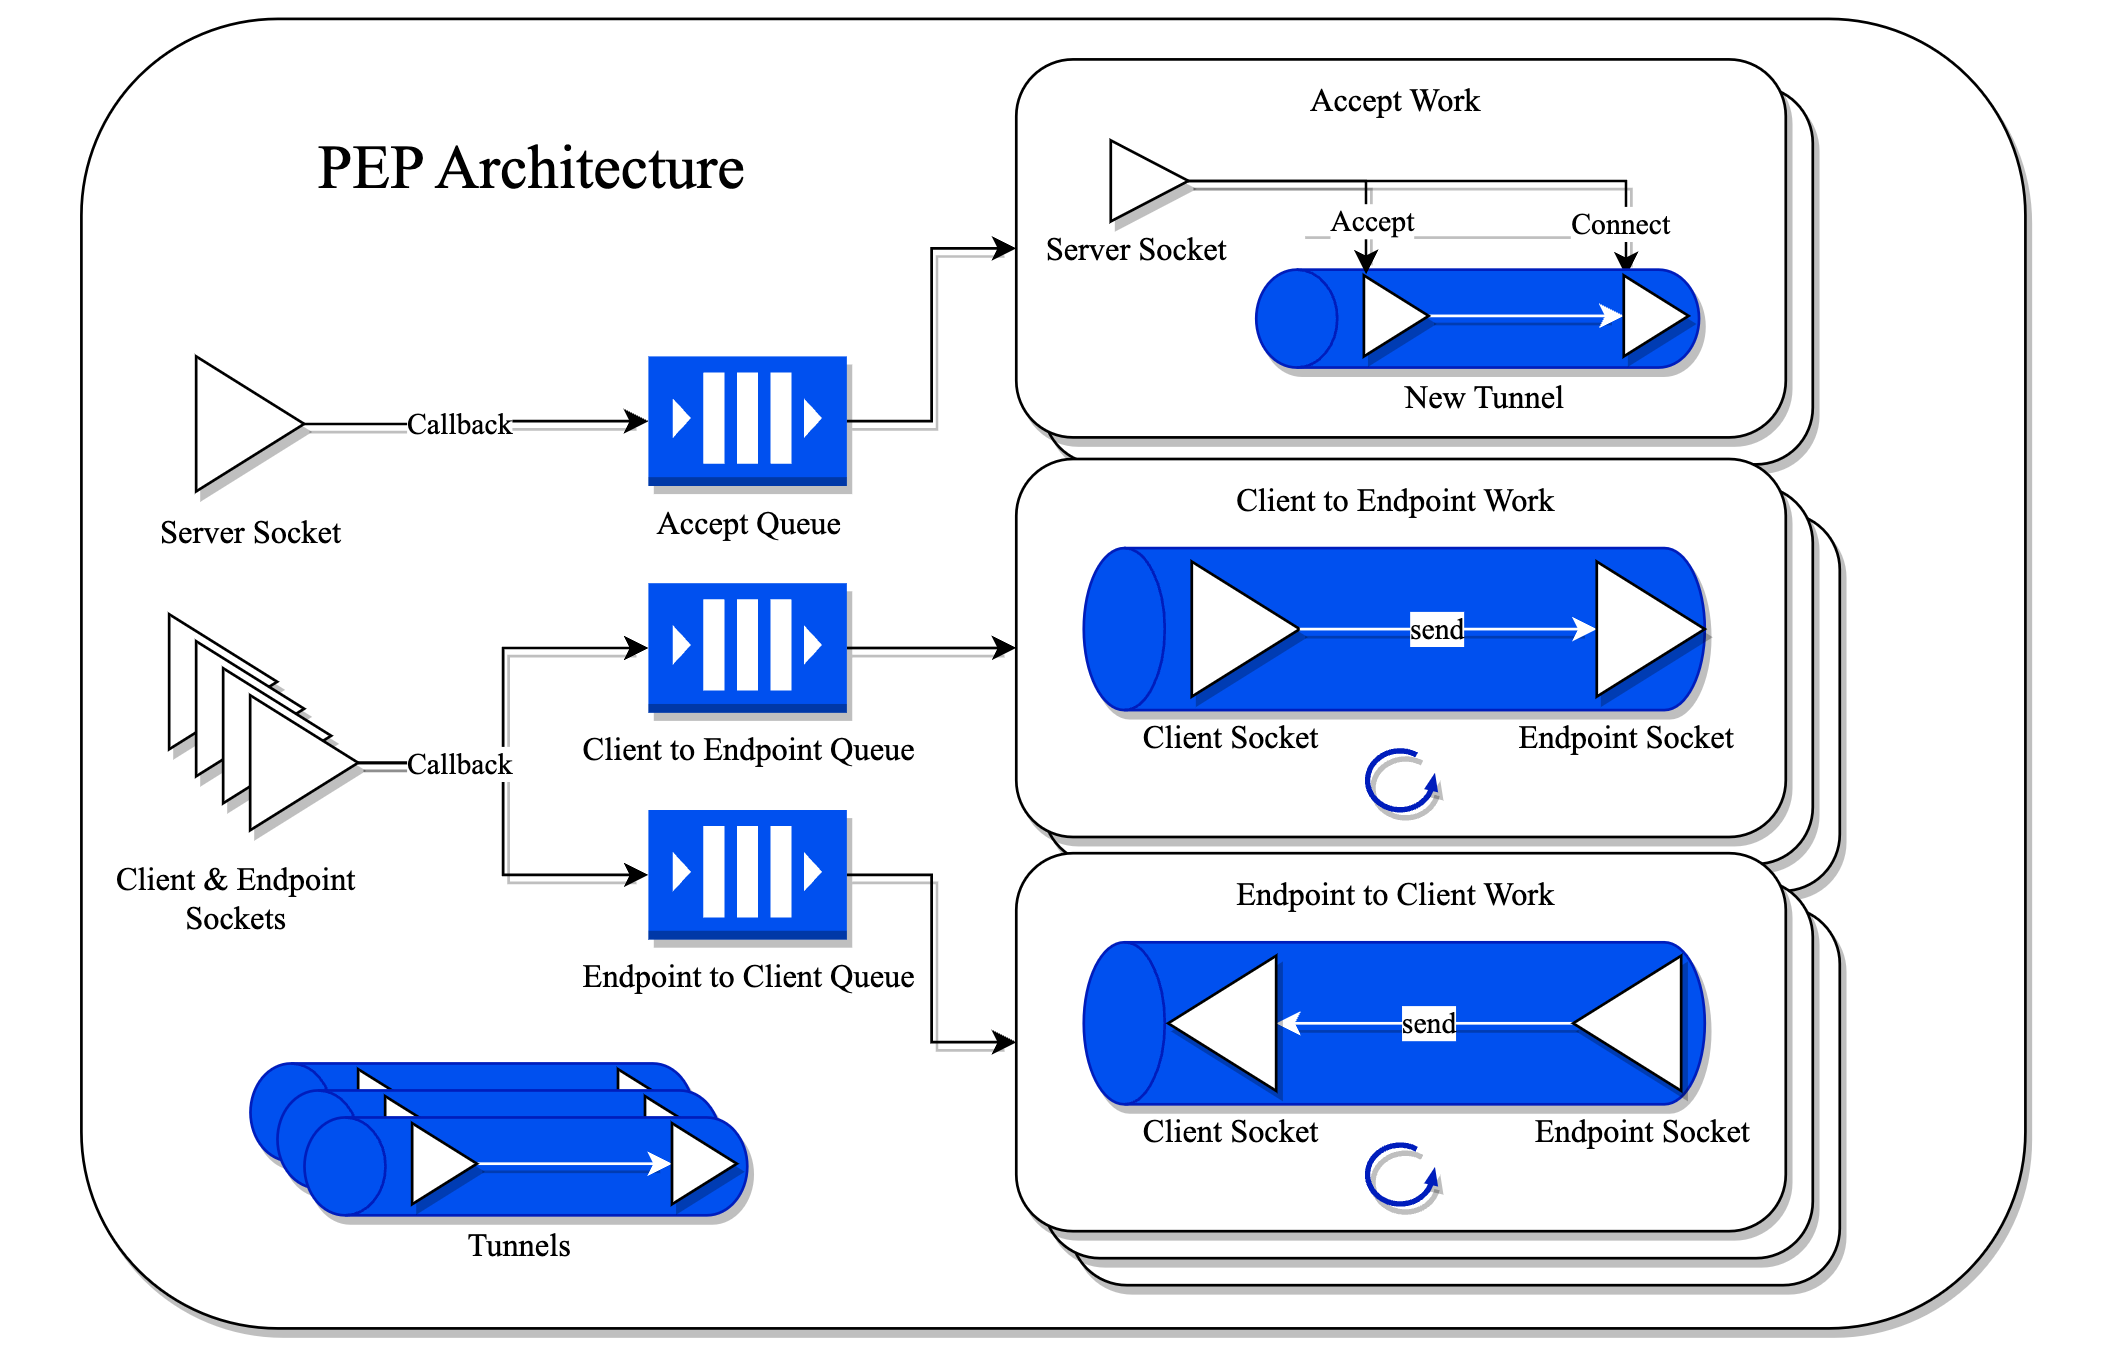
\includegraphics[scale=0.35]{../diagrams/drawio/pep_architecture.png}
  	\caption{The architecture of the PEP}
  	\label{fig:pep_architecture}
\end{figure}

\subsection{Architecture}
The PEPs architecture is mainly based on a server and multiple socket tunnels. The server acts as the entry point of the PEP, clients will connect to the server which will in turn connect to the endpoint. The server consists of a \verb|pep_state| which holds the server socket, work queues and a list of tunnels. The server socket accepts new clients and reads their TLV header, if no header is present the connection will be closed. After successfully reading the TLV, a new socket is created and a connection is attempted to the endpoint specified by the TLVs.\\

\noindent\begin{minipage}{\linewidth}
\begin{verbatim}
struct pep_state {
    atomic_t state;
    
    struct pep_state_ops* ops;
    struct pep_state_work_ops* work_ops;
    
    struct socket* server_socket;
    struct workqueue_struct* accept_wq;
    struct workqueue_struct* forward_c2e_wq;
    struct workqueue_struct* forward_e2c_wq;
    struct work_struct accept_work;
    struct list_head tunnels;
    unsigned int total_tunnels;
};
\end{verbatim}
\captionof{figure}{PEP State Structure Code}
\label{fig:pep_state_structure}
\end{minipage}

\paragraph{Tunnels}
After the endpoint connection is established, the PEP will create a \verb|tunnel|. A \verb|tunnel| consists of 2 sockets, where data is transferred between them. Additionally to the sockets, a \verb|tunnel| also holds the information about the sockets and the proxy connection, this includes total amount of data transferred.\\

\noindent\begin{minipage}{\linewidth}
\paragraph{PEP Tunnel Structure}
\begin{verbatim}
struct pep_tunnel {
        unsigned int id;
        struct pep_connection client;
        struct pep_connection endpoint;
        int total_client;
        int total_endpoint;
        struct work_struct c2e;
        struct work_struct e2c;
        struct list_head list;
        struct pep_state* server;
        int state;
        int recv_callbacks;
        int packets_fowarded;
};
\end{verbatim}
\end{minipage}

[PICTURE OF ARCHITECTURE]\\

\subsection{Kernel Sockets}
Normally an application would interact with socket descriptors when sending and receiving data. However, inside the kernel we have access to the actual sock and socket structures. This gives us full access to all functionality and meta-data a socket can offer, such as \verb|sk_buff| queues, callbacks and statistics like \verb|sk_drops|. An \verb|sk_buff|, which stands for socket buffer, is the kernel struct that holds the information about a packet. It includes both the headers and data and is created when the kernel receives a packet. After that it is routed to the corresponding socket.\\

\noindent\begin{minipage}{\linewidth}
\begin{verbatim}
struct sock {
    atomic_t sk_drops;
    void* sk_user_data;
    ...
    struct sk_buff_head	sk_error_queue;
    struct sk_buff_head	sk_receive_queue;
    ...
    struct socket *sk_socket;
    ...
    void (*sk_state_change)(struct sock *sk);
    void (*sk_data_ready)(struct sock *sk);
    void (*sk_write_space)(struct sock *sk);
    void (*sk_error_report)(struct sock *sk);
    ...
};
\end{verbatim}
\captionof{figure}{Kernel Sock Structure}
\label{fig:kern_sock}
\end{minipage}

\paragraph{Socket Operations}

\paragraph{Socket Callbacks}
Especially of interest is the callback function \verb|sk_data_ready|. It is called whenever a \verb|sk_buff| is received by a socket. That is the case for any kind of packet, not only user data but also includes the TCP handshake packets. This callback can be overwritten by a custom implementation, which is useful to detect any new data on the socket. For example one could inspect or manipulate headers before calling the original \verb|sk_data_ready| function. All callbacks take the socket as a parameters, thereby giving access to the socket state. \\

\paragraph{Socket User Data}
Kernel sockets allow modules to add extra information to a specific socket. The pointer \verb|sk_user_data| can be used to point to any data defined by a module. This in combination with the callbacks is a powerful tool for customizing socket behavior. This allows us to add additional state information to the socket. In our case we will use \verb|sk_user_data| to store the server stat.

Benefit of using kernel moduels -> direct access to socket struct instead of an fd.
socket struct, user\_data, data\_ready callback
Code snippets

\subsection{Work Queues}
To handle multiple concurrent events, the PEP uses \verb|work queues|. A work in the Linux kernel is a way of handling kernel threads. They allow for a more reactive approach to threads, as a work can be queued on demand and execute simple tasks. A work is usually queued into a \verb|work queue|. Each \verb|work queue| represents a task and works which are queued will wait in the queue till they can be run. A task is defined as a function, to which context can be added through a \verb|work| parameter.\\

\noindent\begin{minipage}{\linewidth}
\begin{verbatim}
struct work_struct {
    atomic_long_t data;
    struct list_head entry;
    work_func_t func;
#ifdef CONFIG_LOCKDEP
    struct lockdep_map lockdep_map;
#endif
};
\end{verbatim}
\captionof{figure}{Work struct from Linux - workqueue.h}
\label{fig:work_struct}
\end{minipage}

\subsection{Works}
A work is defined by \verb|work_struct| (see Figure \ref{fig:work_struct}) which holds information associated with the work, most importantly the \verb|work_func_t func|. \verb|func| must be a pointer to a function which takes a \verb|struct work_struct| as parameter. This is the function which will be called when a work is scheduled. The work structure should be created by the user and not be allocated on the stack as external services need access to it. Normally the work structure will be part of another structure as it is in Figure \ref{fig:pep_state_structure}.\\


\begin{autonumlstlisting}[label=lst:work_init]{Work initialization example}
void my_work_handler(struct work_struct *work);

struct work_struct my_work;
struct workqueue_struct * my_workqueue;

my_workqueue = create_singlethread_workqueue("my_workqueue");
INIT_WORK(&my_work, my_work_handler);

queue_work(my_workqueue, &my_work);
\end{autonumlstlisting}

\paragraph{Work state problem}
Initiating a Work poses a challenge: how to effectively track the state. In this context, 'state' refers to the status of a PEP tunnel, which includes the sockets and a reference to the server. A simple approach is to store the PEP server in a global variable. However, not only is this poor coding practice, but it also doesn't solve how to get the sockets. A function that transfers between two sockets must be aware of the specific sockets to use. The work alone doesn't provide this context.\\

To solve this issue we can make use of a macro which Linux provides. \verb|containerof| is a macro that retrieves a reference to the parent structure of any given struct. This in combination with the fact that we do get the original work struct as a parameter.\\

\begin{autonumlstlisting}[label=lst:work_containerof]{Work using containerof example}
struct my_device_data {
    struct work_struct my_work;
    // ...
};

void my_work_handler(struct work_struct *work)
{
   struct my_device_data * my_data;

   my_data = container_of(work, struct my_device_data,  my_work);
   // ...
}
\end{autonumlstlisting}

As described in the PEP Tunnel Structure (see above struct \ref{fig:pep_state_structure}), the PEP has 3 main work queues:
\begin{verbatim}
struct workqueue_struct* accept_wq;
struct workqueue_struct* forward_c2e_wq;
struct workqueue_struct* forward_e2c_wq;
\end{verbatim}

\paragraph{Accept Work Queue}
The main work queue for the server is the accept work queue. When a client attempts a connection to the PEP server we want to receive that notification and queue a accept work. This is an alternative to have a thread blocking on accept. The notification can be achieved by replacing the \verb|sk_data_ready| with a custom function which checks the TCP state and queues a accept work.\\

\begin{autonumlstlisting}[label=lst:pep_accept_callback]{Accept callback function}
void pep_listen_data_ready(struct sock* sk)
{
	struct pep_state* server;

	read_lock_bh(&sk->sk_callback_lock);
	server = sk->sk_user_data;

	/* Queue accept work */
	if(sk->sk_state == TCP_LISTEN){
		queue_work(server->accept_wq, &server->accept_work);
	}
	read_unlock_bh(&sk->sk_callback_lock);

	default_data_ready(sk);
}
\end{autonumlstlisting}

The function \verb|pep_listen_data_ready| (see Listing \ref{lst:pep_accept_callback}) outlines the process of queuing an accept work. We retrieve the PEP server state from the socket \verb|sk_user_data| variable, afterwards we check the socket state for \verb|TCP_LISTEN| which indicates that the socket is ready to accept a connection. If the socket has the correct state we queue the \verb|accept_work| on the \verb|accept_wq| work queue, which is part of the PEP server.

\paragraph{Packet Forwarding Queues}\label{sec:forward_queues}
The second two work queues handle forwarding of packets, one for each direction. The reason we use two separate work and work queues because the function has to identify which socket it should read from and which one it should send to within the tunnel socket pair. \\

[PICTURE PERHAPS?]

\begin{autonumlstlisting}[label=lst:pep_forward_callback]{Forwarding callback function}
void pep_client_data_ready(struct sock* sk)
{
	struct pep_tunnel* tunnel = sk->sk_user_data;
	tunnel->recv_callbacks++;
        
	queue_work(tunnel->server->forward_c2e_wq, &tunnel->c2e);
        
	default_data_ready(sk);
}
\end{autonumlstlisting}

\subsection{Kernel TCP receive and send}
In the kernel, the message functions \verb|recvmsg| and \verb|sendmsg| are used for reading from and sending data to sockets. However, these functions bring some overhead that can lead to code clutter. To reduce this, two helper functions will be utilized instead, \verb|pep_tcp_receive| and \verb|pep_tcp_send|. These functions mimic the usage of the \verb|send| and \verb|recv| system calls, while abstracting away the complexity of the message functions.\footnote{Add these functions as apendix code?}

\begin{verbatim}
int pep_tcp_receive(struct socket *sock, u8* buffer, u32 size);
int pep_tcp_send(struct socket *sock, u8* buffer, u32 size);
\end{verbatim}

The custom functions only take in the socket, buffer and size of buffer as parameters. These functions also abstract away certain error handling which are common in the kernel space such as \verb|EAGAIN| and \verb|ERESTARTSYS|, both of which indicate to retry a function.

\section{PEP - Server}

\subsection{Creation}

\subsection{Server initialization}
Server state initialization consist of creating and configuring the main server socket and work queues. The server is responsible for accepting client and creating pep tunnels. Additionally, it holds the work queues for all the PEPs functionality. Socket configuration consists of replacing the \verb|sk_data_ready| data callback, setting \verb|sk_user_data| to the server itself and using \verb|setsockopt| to set both \verb|TCP_FASTOPEN| and \verb|TCP_NODELAY|. \verb|TCP_NODELAY| is set to avoid socket latency by 'waiting' for larger frames.

\begin{autonumlstlisting}[label=lst:pep_server_init]{PEP server initialization (Simplified)}
int pep_server_init(struct pep_state* server, u16 port)
{
	...

	/* socket creation */
	struct sock* sk = NULL;
	struct sockaddr_in saddr;
	ret = sock_create_kern(&init_net, ..., &sock);
	if(ret){
			printk(KERN_INFO "[PEP] init_core: Error creating socket\n");
			return -EPEP_GENERIC;
	}

	...
	server->state = ((atomic_t){(PEP_SERVER_RUNNING)});
	
	/* use our own data ready function */
	write_lock_bh(&sk->sk_callback_lock);
	sk->sk_user_data = server;
	sk->sk_data_ready = server->callbacks->server_data_ready;
	write_unlock_bh(&sk->sk_callback_lock);

	/* pep server connection info */
	...

	pep_setsockopt(sock, TCP_FASTOPEN, 5);
	pep_setsockopt(sock, TCP_NODELAY, 1);
	
	... bind and listen ...

	server->accept_wq = alloc_workqueue("accept_wq", WQ_HIGHPRI|WQ_UNBOUND, 0);
	server->forward_c2e_wq = alloc_workqueue("c2e_wq", WQ_HIGHPRI|WQ_UNBOUND, 0);
	server->forward_e2c_wq = alloc_workqueue("e2c_wq", WQ_HIGHPRI|WQ_UNBOUND, 0);

	...

	return 0;
}
\end{autonumlstlisting}

Line 20 in Listing \ref{lst:pep_server_init} configures the \verb|sk_data_ready| callback to the before mentioned \verb|pep_listen_data_ready|, when overwriting the \verb|sk_data_ready| we need to make sure we hold the socket \verb|sk_callback_lock| to avoid any race conditions which is done in line 17 and 21. The accept and forward work queues are allocated and created with \verb|WQ_HIGHPRI| and \verb|WQ_UNBOUND|.\\

\noindent\begin{minipage}{\linewidth}
\begin{verbatim}
WQ_HIGHPRI
    Work items of a highpri wq are queued
    to the highpri worker-pool of the target cpu.

WQ_UNBOUND
    Work items queued to an unbound wq are served
    by the special worker-pools which host workers
    which are not bound to any specific CPU.
\end{verbatim}
\captionof{figure}{https://docs.kernel.org/core-api/workqueue.html}
%\label{fig:work_struct}
\end{minipage}\\

The reason for both \verb|WQ_HIGHPRI| and \verb|WQ_UNBOUND| is to avoid any added latency by work queuing, especially if there are a lot of other works being queued. Work queues are used by the kernel for any deferred work, which means that there might be competition for both CPU and scheduling. The before mentioned flags assure that the PEP work's are prioritized.\\

Left out from Listing \ref{lst:pep_server_init} is the creating of the accept work itself. It uses the \verb|INIT_WORK| macro (shown in \ref{lst:work_init}) with the \verb|pep_listen_data_ready| function. After that the server is configured and ready for accept callbacks.

\subsection{Accept and Endpoint connection}
The accept work will call the \verb|pep_server_accept_work| which is responsible for creating a new tunnel and connection to the desired endpoint. First the server state is fetched by using \verb|container_of|, after which we assert that the server is in a operational state. Next, the kernel will accept a new connection in a non-blocking fashion as we know there is a incoming connection request.\\

\begin{autonumlstlisting}[label=lst:pep_server_accept]{PEP server accept function (Simplified)}
int pep_server_accept_work(struct work_struct *work)
{
    struct pep_state* server = container_of(work, struct pep_state, accept_work);

    rc = kernel_accept(server->server_socket, ...);
    
    ... read data from socket ...

    /* Validate tlv header. */
    if(!tlv_validate(buffer)){
        return;
    }
    
    /* Get connect tlv options from tlv buffer */
    tlv = tlv_get_option(TLV_CONNECT, buffer);
    if(tlv == NULL || tlv->length != 6){
        sock_release(client);
        return; 
    }

    endpoint = pep_endpoint_connect(tlv->optional, tlv->value);
    if(NULL == endpoint){
        sock_release(client);
        return; 
    }
    
    ... configure sockets and tunnel ...
    
    return 0;
}
\end{autonumlstlisting}


After successfully accepting the client we immediately allocate a buffer and read from the client. We expect it to send a TLV with TCP Fast Open, so we use the TLV library to validate and read the TLV options. Note that even if TCP Fast Open should fail the connection can still be established at the cost of the additional round trip times. Specifically we look for the \verb|TLV_CONNECT| option, which will be used to connect to the endpoint.\\

\subsection{Multiple Servers}
Because of the callback nature of the PEP we can create multiple servers on the same host machine. By not having a 'global' server in the kernel module, we are able to potentially create as many servers as we want\footnote{Should I use "we want"?}. The programmer only has to keep track of the server pointers, while the implementation of the server keeps track of the states and correct callback handling through the works. This means that each server may use the same callback function, but the state will vary.

\section{PEP - Clients}

\subsection{Client Sockets - Endpoint Sockets}
As discussed in Section \ref{sec:forward_queues}, there are two functions responsible for forwarding packets. After queuing a forwarding work from a callback, the corresponding function is executed.

\begin{autonumlstlisting}[label=lst:pep_forward]{Client Forwarding Function (Simplified)}
void pep_client_receive_work(struct work_struct *work)
{
	int ret = 1;
	int ret_forward;
	struct pep_tunnel* tun = container_of(work, struct pep_tunnel, c2e);

	unsigned char *buffer = kzalloc(...);
	if (!buffer) {
		return;
	}

	while(ret > 0){
		ret = pep_tcp_receive(tun->client.sock, ...);
		if(ret > 0){
			ret_forward = pep_tcp_send(tun->endpoint.sock, ...);
			tun->total_client += ret_forward;
			tun->packets_fowarded++;
		} else {
			if(pep_tunnel_is_disconnected(tun)){
				pep_tunnel_close(tun);
				return;
			}
		}
	kfree(buffer);
}
\end{autonumlstlisting}

Listing \ref{lst:pep_forward} shows the function that forwards data from the client to a endpoint. First we retrieve the tunnel state by using \verb|container_of|, this gives us the sockets which triggered the original callback. After that, a buffer is allocated and data is read from the client and forwarded to the endpoint. This function will run while there is data to send, the reason is that it is more effect to read all the data that is available than to wait for a callback and work queue to trigger.\\

If a socket returns 0 or less we check if the connection is closed, that is because the closing of a connection will trigger the same \verb|sk_data_ready| callback. However, when a socket is closed it will return 0 or an appropriate error code. (How shutdown is done, RW, WR, etc)

\subsection{PEP Connections}
By design the PEP is able to handle multiple connections at once. Each socket pair has its own work structure for client - endpoint and endpoint - client communication. This means, each work structure can run in parallel, in both directions. Each tunnel (socket pair) is added to a linked list in the server state. Meaning we have access to them in case we need to prematurely terminate the connections. This will avoid any memory leaks since we manage the memory for the tunnels.\\

\subsection{Module Customization}
The PEP will follow a similiar approach as congestion control when it comes to how the PEP is configured. The basic accept and forward functions will be defined by a table, which can be created by any future model. Each server has a pointer to this table, which it uses when creating works. This mimics the way we configure socket callbacks and makes each PEP server more customizable. Each individual PEP server can have different forward functions, or keep the orignal ones.\\\\

\noindent\begin{minipage}{\linewidth}
\begin{verbatim}
struct pep_state_work_ops {
    void (*accept)(struct work_struct *work);
    void (*forward_c2e)(struct work_struct *work);
    void (*forward_e2c)(struct work_struct *work);
};
\end{verbatim}
\captionof{figure}{Work operation table}
%\label{fig:work_struct}
\end{minipage}\\

The work function table in combination with the fact that the PEP supports multiple servers, means that each indiviudal server can be configured different without needing to change any of the original code. Simply creating a new \verb|struct pep_state_work_ops| and supplying new work functions is enough:\\

[EXAMPLE CODE]\footnote{Talk about callback table too}

\noindent\begin{minipage}{\linewidth}
\begin{verbatim}
struct pep_socket_callbacks {
    void (*server_data_ready)(struct sock* sk);
    void (*client_data_ready)(struct sock* sk);
    void (*endpoint_data_ready)(struct sock* sk);
};
\end{verbatim}
\captionof{figure}{Callback function table}
%\label{fig:work_struct}
\end{minipage}\\

\subsection{System Configurations}
The PEP will require some configuration outside of the kernel module itself. Linux uses \verb|sysctl| for system configuration. Most importantly we want to enable TCP Fast Open and IP forwarding, IP forwarding will allow the Linux machine to act as a router and forward packets, which is important as the PEP will handle all other traffic as well. Both these options are under \verb|net.ipv4| ...\\

\begin{verbatim}
$ sysctl -w net.ipv4.tcp_fastopen=3
$ sysctl -w net.ipv4.ip_forward=1 
\end{verbatim}

\paragraph{Buffer sizes}
The PEP works by buffering as much data as possible on the sockets themselves. This way we avoid buffering interactive traffic that simply passes by. The size of a socket's buffer can be configured with \verb|setsockopt|, however this is not reliable and has to be done for each socket. Instead we can configure the socket buffer sizes system-wide. Under \verb|net.core| there exists configurations for overall receive buffer sizes: \verb|rmem_max| and \verb|wmem_max|. There also exists the same for the default variables \verb|rmem_default| and \verb|wmem_default|.\\

\begin{verbatim}
$ sudo sysctl -w net.core.rmem_max=<size>;
$ sudo sysctl -w net.core.wmem_max=<size>;
$ sudo sysctl -w net.core.rmem_default=<size>;
$ sudo sysctl -w net.core.wmem_default=<size>;
\end{verbatim}

Additionally, under \verb|net.ipv4| there are options to configure the amount of memory in bytes a TCP socket can buffer for both total, read and write. Each contains three numbers: the minimum, default, and maximum values.

% [https://wiki.linuxfoundation.org/networking/tcp_memory_documentation]

\begin{verbatim}
$ sudo sysctl -w net.ipv4.tcp_rmem='<min size> <size> < max size>';
$ sudo sysctl -w net.ipv4.tcp_wmem='<min size> <size> < max size>';
$ sudo sysctl -w net.ipv4.tcp_mem='<min size> <size> < max size>';
\end{verbatim}

\subsection{Userspace?}
Could this be implemented in user-space?

\subsection{Threads Vs. Callbacks}
Small discussion around that?


\subsection{Using Netfilter}
Forwarding using Netfilters, why we dont want this.


\section{Memory}
Memory Management in C, why its important, how we deal with it.

\chapter{Evaluation}
Our evaluation of the PEP centers on measuring the completion times for non-interactive traffic. We aim to demonstrate how the PEP can speed up this traffic compared to standard end-to-end methods. It's also important that this enhancement doesn't negatively affect interactive traffic. To illustrate this, we'll use graphs to show the impact on interactive traffic.

We will begin with a basic test case to understand how well the PEP works in a simple scenario. After that we will look at how the PEP handles situations with changing bandwidth, which is more common in real-world settings.

\section{Testbed}
The testbed consists of multiple machines running Debian linux..
A central controller is used to orchestrate the experiments.

\section{Ultra Ping}
Ultra ping is a tool for characterizing UDP packet latency in a network. The tool measures the time it takes for UDP packets to get across the network\cite{rahtz2023ultraping}. We will use Ultra Ping to simulate interactive traffic and have it compete with the PEP. Additionally, Utra Ping provides tools for plotting and creating graphs of the measured data.\\

Ultra Ping lets you configure the amount of packets, packet size and sending rate in kBps. For our evaluation we will use... which mimics Skype.

\begin{verbatim}
./echo.py --server
./echo.py --client <IP address of server>
\end{verbatim}

\section{Initial configuration}
The initial test configuration will consist of a Sender, Receiver and the PEP. Where the Sender is connected to the PEP and the PEP connected to the Receiver. Each point is a Linux host running Debian, directly interconnected with Ethernet cables.\\

\begin{figure}[h!] % htbp stand for "here", "top", "bottom", "page"
	\centering
	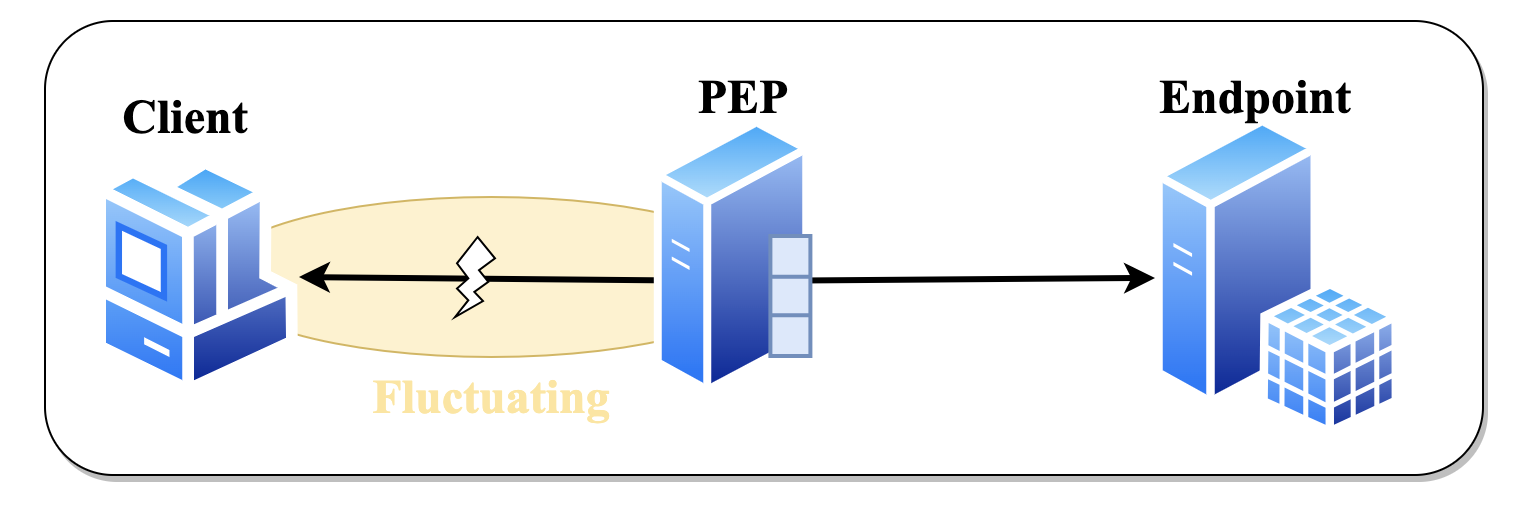
\includegraphics[scale=0.45]{../diagrams/drawio/simple_pep_design.png}
  	\caption{PLACEHOLDER}
  	\label{fig:inital_configuration}
\end{figure}

In this configuration data will be sent from the sender to the receiver, non-interactive traffic data will go through the PEP while the interactive Ultra Ping data will only be routed by the PEP. The connection between Sender and PEP will represent the stable network while the connection between the PEP and Receiver will represent a unstable wireless network.

\subsection{Traffic Control Options}
Linux has support for network interface configurations using the TC (traffic control) command. TC allows the configuration of packet scheduler, bandwidth, delay and jitter etc. These options combined with the fact that each network interface can have it's own configuration, allows for very precise testing environments. 
\\
fq codel does not allow the configuration of delay, this means we have to configure the delay on the path of the ACKS?
We have to configure the delay on sender facing interface cards. 
\footnote{Picture of testbed setup} 

\subsection{Scheduling Algorithms}
The choice of scheduling algorithm is very important for our test scenarios. As it will greatly affect the results of our tests, we will compare some against each other. The main goal is to highlight the effect and find the optimal algorithms for our PEP.

\paragraph{FIFO}
In our test case FIFO will have the effect of creating up a queue at our PEP. This is detrimental for the interactive UDP flow as it will be stuck in the queue, building up delay. This behavior can be explained by the fact that the non-interactive flow has a much higher sending rate than the interactive flow, thereby quickly filling the finite queue with non-interactive packets.

\paragraph{FQ CoDel: IMPORTANT}
FQ CoDel has a solution for this problem by providing a fair queuing mechanism. 
\paragraph{PFIFO}
Another alternative is Priority FIFO (PFIFO). As the name suggests it combines the concepts of a basic FIFO queue with priorities. This can reduce delay


\subsection{Interactive vs PEP}
Our first experiment consists of having a interactive flow (100 byte UDP packets at 2kBps) competing with a file transfer, one default end to end and one through our PEP. Highlighting some of the initial differences between an end to end connection and a PEP.\\


\begin{figure}[h] % htbp stand for "here", "top", "bottom", "page"
	\centering
	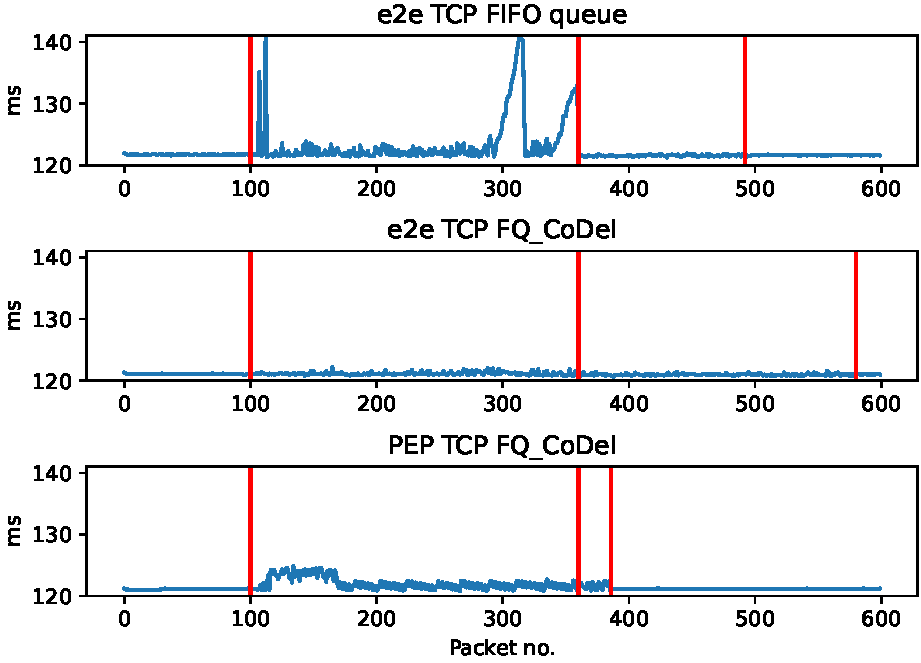
\includegraphics[scale=0.50]{../diagrams/graphs/initial_udp_latency_timeseries.pdf}
  	\caption{Interactive UDP traffic}
  	\label{fig:inital_test}
\end{figure}

\subsection{PEP vs E2E tests}
The first test consists of evaluating our PEP against a default TCP end to end (E2E) connection, while also highlighting the difference a packet scheduler can make. Fig. \ref{fig:inital_test} shows the results, the red lines represent important events in the time-line.
The first line represents the start of a file transfer, the second shows a bandwidth change from 10mbit to 75mbit, while the last line shows when the file transfer finished.\\ 

The first time-line shows an end to end TCP transfer using a FIFO queue, in this case BFIFO.\\ 
On the second timeline we see the behavior of an end to end connection using FQ CoDel. {MORE}
The last timeline shows the PEP using FQ CoDel. Looking at the graph we can see two important differences between the default end to end TCP and the PEP. Firstly, the PEP has higher latency fluctuations than the E2E connection, shown by the blue liens on the graph. 

% FIGURE OF THE TEST SETUP

\subsection{10x10 tests}
To further evaluate the PEP we conducted an experiment where we have 1-10 flows competing, once using the PEP and once end to end. The goal is to see how competing flows affect the behavior of or PEP

\subsection{Spike}

\chapter{Conclusion}
	
\chapter{New Testing}
To evaluate the initial performance of the PEP we use a simple topology consisting of a sender, router and a sender. The router will act as our hypothetical base station at which the PEP resides. The connection between the router and the receiver will act as the unstable fluctuating bandwidth domain.\footnote{Rewrite this part}\\

Sender -(100Mbit, 100ms)- Router -(15mbit, 20ms)- Receiver\\

The goal is to confirm the two most important aspects of the PEP, a faster completion time and no interference with the interactive traffic. To achieve this we will send a 32 megabyte file from the sender to the receiver, while simultaneously have a interface UDP traffic (how fast and how much). The interactive data will simulate Skype traffic using a program called ULTRA\_PING which offer end to end latency measurements.\\

Fluctuating bandwidth is simulated by a step function.\\

<graph>\\

The first graph shows 3 interactive flows each competing with a file transfer. The first is a normal end to end transfer using a FIFO (bfifo) queue at the router. The second is an end to end transfer using FQ\_CODEL, and the last is the same transfer with the PEP.\\

\section{Configuration}
TC, TSO, scheduling, delay.


\subsection{Experiment 1}



\section{File transfer}
The file transfer is simulated by a two custom C programs. Using a command line argument you specify if the Sender uses the pep\_connect or connect function. The reason for creating custom C programs is that we need to use the TLV library for connecting to the PEP. The sender will use the default socket API sending 1500 bytes at a time. The receiver is responsible for receiving the data and keep track of the time it took. The receiving server can handle multiple file transfers at the same time using threads.

\section{Results}

\section{Future Work}

\bibliography{myBib.bib}{}
\bibliographystyle{plain}
\end{document}
